\documentclass[11pt,oneside]{book}
\usepackage{amsmath}
\usepackage{amssymb}
\usepackage{amsthm}
\usepackage{amsfonts}
\usepackage{multirow}
\usepackage{float}
\usepackage{diagbox}
\usepackage{xcolor}
\usepackage{caption}
\usepackage{graphicx}
\usepackage{subfigure}
\graphicspath{{img/}}
\usepackage{paralist}
\usepackage{tikz}
\let\itemize\compactitem
\let\enditemize\endcompactitem
\let\enumerate\compactenum
\let\endenumerate\endcompactenum
\let\description\compactdesc
\let\enddescription\endcompactdesc
\setlength{\parindent}{0pt}
\title{Notes of Mathematical Analysis}
\author{}
\date{}
\newtheorem{theorem}{Theorem}[section]
\newtheorem*{lemma}{Lemma}
\newtheorem{definition}{Definition}[section]
\theoremstyle{definition}
\newtheorem{ex}{Exercise}[section]
\newtheorem*{answer}{Answer}
\newcommand\thmref[1]{\textbf{Theorem \ref{#1}}}
\newcommand\figref[1]{\textbf{Figure \ref{#1}}}
\begin{document}
\newtheorem*{tips}{\emph{TIPS}}
\chapter{Groups}
\section{Semigroups, monoids and groups}
\begin{ex}
    Give examples other than those in the text of semigroups and monoids that are not groups.
\end{ex}

\begin{answer}
    Semigroup: $(\mathbf{Z}_+, +)$

    Monoid: $(\mathbf{Z}_+, \times )$ 
\end{answer}

$$ $$

\begin{ex}
    Let $G$ be a group (written additively), $S$ a nonempty set, and $M(S,G)$ the set of all functions $f: S \rightarrow G$. Define addition in $M(S,G)$ as follows: $(f + g) : S \rightarrow G$ is given by $s \rightarrow f(s) + g(s) \in G$. Prove that $M(S,G)$ is a group, which is abelian if $G$ is.
\end{ex}

\begin{answer}
    Firstly we check $M(S,G)$ is a group
    \begin{enumerate}
        \item $f+g: s\to f(s) + g(s) \in G$, so $f+g\in M(S,G)$
        \item $(f+g)+h: s\to (f(s) + g(s)) + h(s)$, $G$ is a group, so $s\to (f(s) + g(s)) + h(s)\Leftrightarrow s\to f(s) + (g(s) + h(s))$, $(f+g)+h = f+(g+h)$.
        \item Take the unit element as $e': s\to e$. $f+e': s\to f(s)+ e'(s) =f(s)+e=f(s)$, so $f+e'=f$. Similarly, $e'+f = f$.
        \item For any $f\in M(S,G)$, take $f^{-1}: s\to (f(s))^{-1}$, whence $f(s)+(f(s))^{-1}=(f(s))^{-1}+f(s)=e$.
    \end{enumerate}
    In conclusion, $M(S,G)$ is a group. If $G$ is abelian $f+g: s\to f(s)+g(s)=g(s)+f(s)$, $f+g=g+f$, so $M(S,G)$ is abelian.
\end{answer}

$$ $$

\begin{ex}
    Is it true that a semigroup which has a left identity element and in which every element has a right inverse (see Proposition 1.3) is a group?
\end{ex}

\begin{answer}
    If $e$ is the left identity, $\forall a \in A, ea=a$ and $\forall a\in A ,\exists  a^{-1} s.t. aa^{-1}=e$. We have proved that if $cc=c$, then $c=e$. \[(a^{-1}a)(a^{-1}a)=a^{-1}(aa^{-1})a=a^{-1}(ea)=a^{-1}a\Rightarrow a^{-1}a=e\]
    $a^{-1}$ is also the left inverse. $ae=a(a^{-1}a)=(aa^{-1})a=ea=a$, $e$ is also the right identity.
\end{answer}

$$ $$

\begin{ex}
    Write out a multiplication table for the group $D_4^*$.
\end{ex}

\begin{answer}
    $D_4^*=\{R,R^{2}, R^{3},I,T_x,T_y,T_{13},T_{24}\}$
    \begin{table}[H]
        \centering
        \begin{tabular}{c|cccccccc}
        \multicolumn{1}{c}{} & $I$ & $R$ & $R^{2}$ & $R^{3}$ & $T_x$ & $T_y$ & $T_{13}$ & $T_{24}$  \\ 
        \cline{2-9}
        $I$ & $I$ & $R$ & $R^{2}$ & $R^{3}$ & $T_x$ & $T_y$ & $T_{13}$ &  $T_{24}$ \\
        $R$ & $R$ & $R^{2}$ & $R^{3}$ & $I$ & $T_{13}$ & $T_{24}$ & $T_y$ & $T_x$  \\
        $R^{2}$ & $R^{2}$ & $R^{3}$ & $I$ & $R$  & $T_y$ & $T_x$ & $T_{24}$ & $T_{13}$  \\
        $R^{3}$ & $R^{3}$ & $I$ & $R$  & $R^{2}$ & $T_{24}$ & $T_{13}$ & $T_x$ & $T_y$  \\
        $T_x$ & $T_x$ & $T_{24}$ & $T_y$ & $T_{13}$ & $I$ & $R^{2}$ & $R^{3}$ & $R$  \\
        $T_y$ & $T_y$ & $T_{13}$ & $T_x$ & $T_{24}$ & $R^{2}$ & $I$ & $R$ & $R^{3}$  \\
        $T_{13}$ & $T_{13}$ & $T_y$ & $T_{24}$ & $T_x$ & $R^{3}$ & $R$ & $I$ &  $R^{2}$ \\
        $T_{24}$ & $T_{24}$ & $T_x$ & $T_{13}$ & $T_y$ & $R$ & $R^{3}$ & $R^{2}$ &  $I$
        \end{tabular}
        \end{table}
\end{answer}

$$ $$

\begin{ex}
    Prove that the symmetric group on $n$ letters, $S_n$, has ordrer $n!$.
\end{ex}

\begin{answer}
    For a set $A$ whose order is $n$, we prove there's $n!$ different bijections by induction
    \begin{enumerate}
        \item For $n=1$, trivial.
        \item Assume $n=k$, there's $k!$ bijections. For $n=k+1$m fix one element in $A$, and take $a\to a$, there's $k$ free elements, so there's $K!\cdot(k+1)$ bijections in total.
    \end{enumerate}
    By induction, we get the result.
\end{answer}

$$ $$

\begin{ex}
    Write out an addition table for $Z_2\oplus Z_2$. $Z_2\oplus Z_2$ is called the Klein four group.
\end{ex}

\begin{answer}
    $Z_2=\{1,0\}$, $Z_2\oplus Z_2=\{(1,1), (1,0), (0,1), (0,0)\}$
    \begin{table}[H]
        \centering
        \begin{tabular}{c|cccc}
            \multicolumn{1}{c}{} & $(1,1)$ & $(1,0)$ & $(0,1)$ & $(0,0)$\\
            \cline{2-5}
            $(1,1)$ & $(0,0)$ & $(0,1)$ & $(1,0)$ & $(1,1)$ \\
            $(1,0)$ &$(0,1)$  & $(0,0)$ & $(1,1)$ & $(1,0)$ \\
            $(0,1)$ & $(1,0)$ & $(1,1)$ & $(0,0)$ & $(0,1)$ \\
            $(0,0)$ & $(1,1)$ & $(1,0)$ & $(0,1)$ & $(0,0)$
        \end{tabular}
    \end{table}
\end{answer}

$$ $$

\begin{ex}
    If $p$ is prime, then the nonzero elements of $Z_p$ form a group of order $p - 1$ under multiplication. Show that this statement is false if $p$ is not prime.
\end{ex}

\begin{answer}
    For the set $Z_p\backslash\{\bar{0}\}$
    \begin{enumerate}
        \item $Z_p\backslash\{\bar{0}\}$ is obviously associative and communicative.
        \item Take $\bar{1}$ as the identity element, $\forall \bar{a}\in Z_p\backslash\{\bar{0}\}, \bar{1}\times \bar{a}=\bar{a}$.
        \item We prove there is a unique element $a^{-1}\in Z_p\backslash\{\bar{0}\} s.t. aa^{-1}=\bar{1} $. Assume there exists $\bar{b},\bar{c}$ and $\bar{a}\cdot\bar{b}=\bar{k},\bar{a}\cdot\bar{c}=\bar{k}$, then $a(b-c)\equiv 0\mod{p}$. $p$ is a prime, so $lcm(p,a)=1,  lcm(p,b-c)=1$, so $\bar{b}=\bar{c}$. There is at most one element s.t. $\bar{a}\bar{b}=\bar{k}$. Take $\bar{b}=\bar{1}, \bar{2},\dots\bar{p-1}$, $\bar{k}$ travels through $\bar{b}=\bar{1}, \bar{2},\dots\bar{p-1}$. There exists an element $\bar{b}\in Z_p\backslash\{\bar{0}\}, \bar{a}\bar{b}=\bar{1}$.
    \end{enumerate}
    $Z_p\backslash\{\bar{0}\}$ is a group. If $p$ is not a prime, the inverse element is not always unique. Take $a|p$, there's more than one inverse element in $Z_p\backslash\{\bar{0}\}$.
\end{answer}

$$ $$

\begin{ex}
    \begin{enumerate}
        \item The relation given by $a ~ b \Leftrightarrow a - b \in \mathbf{Z}$ is a congruence relation on the additive group $\mathbf{Q}$ [see Theorem 1.5].
        \item The set $\mathbf{Q}/\mathbf{Z}$ of equivalence classes is an infinite abelian group.
    \end{enumerate}
\end{ex}

\begin{answer}
    \begin{enumerate}
        \item For group $(\mathbf{Q}, +)$, $a_1~b_1\Leftrightarrow a_1-b_1=k_1\in \mathbf{Z}$, $a_2~b_2\Leftrightarrow a_2-b_2=k_2\in \mathbf{Z}$, so $(a_1+a_2)-(b_1+b_2)=((k_1+b_1)+(k_2+b_2))-(b_1+b_2)=k_1+k_2\in\mathbf{Z}$. $a~b$ is a congruence relation.
        \item \begin{enumerate}[1]
            \item if $a+b\geq 1$, $\bar{a}+\bar{b}=\bar{a+b-1}$. If $a+b<1$, $\bar{a}+\bar{b}=\bar{a+b}$.
            \item $\mathbf{Q}/\mathbf{Z}$ is obviously associative and communicative.
            \item Take the identity element as $\bar{0}$, $\bar{0}+\bar{a}=\bar{a}$.
            \item If $\bar{a}\neq 0$, take $(\bar{a})^{-1}=\bar{1-a}$, then $\bar{a}+\bar{1-a}=\bar{0}$
        \end{enumerate}
        so $\mathbf{Q}/\mathbf{Z}$ is a abelian group. (Infinite remains to be certified)
    \end{enumerate}
\end{answer}

$$ $$

\begin{ex}
    Let $p$ be a fixed prime. Let $R_p$ be the set of all those rational numbers whose denominator is relatively prime to $p$. Let $R^p$ be the set of rationals whose denominator is a power of $p (p^i, i > 0)$. Prove that both $R_p$ and $R^p$ are abelian groups under ordinary addition of rationals.
\end{ex}

\begin{answer}
    Trivial.
\end{answer}

$$ $$

\begin{ex}
    Let $p$ be a prime and let $Z(p^\infty)$ be the following subset of the group $\mathbf{Q}/\mathbf{Z}$:\[Z(p^\infty)=\{\bar{a/b}\in\mathbf{Q}/\mathbf{Z}| a,b \in \mathbf{Z} \text{ and } b=p^i \text{ for some }i\geq 0\}\]
    Show that $Z(p^\infty)$ is an infinite group under the addition operation of $\mathbf{Q}/\mathbf{Z}$.
\end{ex}

\begin{answer}
    $Z(p^\infty)=\{\bar{a/b}|a, b\in\mathbf{Z}, b=p^i, i\geq 0 \}$. Take $a=\bar{\frac{a_1}{b_1}}$, $b=\bar{\frac{a_2}{b_2}}$. $b^{-1}=\bar{\frac{b_2-a_2}{b_2}}$
    \[\begin{aligned}
        a+b^{-1}=\bar{\frac{a_1}{b_1}}+\bar{\frac{b_2-a_2}{b_2}}&=\bar{\frac{a_1}{p^{s_1}}}+\bar{\frac{p^{s_2}-a_2}{p^{s_2}}}\\ &=\bar{\frac{a_1\cdot p^{s_2}+p^{s_1}(p^{s_2}-a_2)}{p^{s_1+s_2}}}\in Z(p^\infty)
    \end{aligned}\]
    Therefore, $Z(p^\infty)$ is a subgroup of $\mathbf{Q}/\mathbf{Z}$. $\frac{1}{p^i}\in Z(p^\infty)$ for any $i \in \mathbf{Z}$, so $Z(p^\infty)$ is infinite, $\mathbf{Q}/\mathbf{Z}$ is also infinite.
\end{answer}

$$ $$

\begin{ex}
    The following conditions on a group $G$ are equivalent:
    \begin{enumerate}[i]
        \item $G$ is abelian;
        \item $(ab)^2=a^{2}b^{2}$ for all $a,b\in G$;
        \item $(ab)^{-1}=a^{-1}b^{-1}$ for all $a,b \in G$;
        \item $(ab)^{n}=a^{n}b^{n}$ for all $n\in \mathbf{Z}$ and all $a,b \in G$;
        \item $(ab)^{n}=a^{n}b^{n}$ for three consecutive integers $n$ and all $a,b \in G$. Show that v$\Rightarrow$ i is false if `three' is replaced by `two'.
    \end{enumerate}
\end{ex}

\begin{answer}
    i$\Leftrightarrow$ iii: $((ab)b^{-1})a^{-1}=(ab)(b^{-1}a^{-1})=e$, so $(ab)^{-1}=b^{-1}a^{-1}$. If iii, $b^{-1}a^{-1}=a^{-1}b^{-1}$ for any $a,b \in G$, $G$ is abelian. If i, $G$ is abelian, $(ab)^{-1}=b^{-1}a^{-1}=a^{-1}b^{-1}$.

    iv $\Rightarrow$ v, iv$\Rightarrow$ ii and i$\Rightarrow$ iv are trivial.

    ii$\Rightarrow$ i: \[(ab)(ab)=aabb\Rightarrow a^{-1}(ab)^{2}b^{-1}=a^{-1}aabbb^{-1}=ba=ab\] so $G$ is abelian.

    v $\Rightarrow$ i: $a^{n}b^{n}=(ab)^{n}$, $a^{n-1}b^{n-1}=(ab)^{n-1}$, $a^{n+1}b^{n+1}=(ab)^{n+1}$. \[(b^{-1})^{n}(a^{-1})^{n}=((ab)^{n})^{-1}=((ab)^{-1})^{n}\]\[((ab)^{-1})^{n}(ab)^{n+1}=(b^{-1})^{n}ab^{n+1}\]\[((ab)^{-1})^{n}(ab)^{n-1}=b^{-1}a^{-1}=(b^{-1})^{n}a^{-1}b^{n-1}\]\[a=(b^{-1})^{n}ab^{n}\qquad b^{-1}a^{-1}b=(b^{-1})^{n}a^{-1}b^{n}\]So $a^{-1}=b^{-1}a^{-1}b$, which means $G $ is abelian.

    If ``three'' is replaced by ``two'': $a^{n}b^{n}=(ab)^{n}$, $a^{n+1}b^{n+1}=(ab)^{n+1}$. \[(b^{-1})^{n}(a^{-1})^{n}=((ab)^{-1})^{n}\qquad a=(b^{-1})^{n}ab^{n}\] 
    For the group $S_3=\{(1),(12),(13),(23),(123),(132)\}$, taking any $a\in S_3$, we can check that $a^{6}=(1)$. If $n=6$, then $a=(b^{-1})^{n}ab^{n}$ for any $a,b \in S_3$. But $S_3$ is nonabelian.
\end{answer}

$$ $$

\begin{ex}
    If $G$ is a group, $a,b\in G$ and $bab^{-1}=a^{r}$ for some $r\in \mathbf{N}$, then $b^{j}ab^{-j}=a^{r^{j}}$ for all $j\in \mathbf{N}$. 
\end{ex}

\begin{answer}
    $bab^{-1}= a^{r}$. We prove it by induction. For $j=1$, its always true. Assume $j=k$ the equation is correct, $b^{k}ab^{-k}=a^{r^{k}}$. $ba^{r^{k}}b^{-1}=(a^{r^{k}})^{r=a^{r^{k+1}}}$. For $j=k+1$, it's also true.
\end{answer}

$$ $$

\begin{ex}
    If $a^{2}=e$ for all elements $a$ of a group $G$, then $G$ is abelian.
\end{ex}

\begin{answer}
    \[a^{2}=e\Rightarrow a^{2}a^{-1}=ea^{-1}=a(aa^{-1})=ae\Rightarrow a=a^{-1}\]\[ab=a^{-1}b^{-1}=(ab)^{-1}=(ba)^{-1}\]So  $ab=ba \forall a,b \in G$. $G$ is abelian.
\end{answer}

$$ $$

\begin{ex}
    If $G$ is a finite group of even order, then $G$ contains an element $a\neq e$ such that $a^{2}=e$.
\end{ex}

\begin{answer}
    Suppose not. $\forall a\neq e, aa\neq e \Leftrightarrow a\neq a^{-1}$. We can classify the group into some subsets. $G=\bigcup\limits_{a\neq e}\{a,a^{-1}\}\cup\{e\}$. Notice that $\{a,a^{-1}\}\cap\{b,b^{-1}\}=\oslash$ if $a\neq b$, so $\left| G \right| =2n+1$, That's contradictory!
\end{answer}

$$ $$

\begin{ex}
    Let $G$ be a nonempty finite set with an associative binary operation such that for all $a, b, c\in G$, $ab = ac\Rightarrow b = c$ and $ba  =ca \Rightarrow b = c$. Then $G$ is a group. Show that this conclusion may be false if $G$ is finite.
\end{ex}

\begin{answer}
    $G$ is a semigroup. Fix $a\in G$ and take $b$ travels through all elements in $G$, then $ab$ travels through all elements in $G$.

    There exists an element $e_1$ s.t. $ae_1=a\forall a\in G$. Similarly, we can find $e_2$ s.t. $e_2a=a\forall a\in G$. $e_2e_1=e_1=e_2=e$. $e$ is the identity element of $G$. Easily, we can find that $\forall a\in G, \exists ! a^{-1}\in G$ s.t. $a^{-1}a=aa^{-1}=e$ because $ab = ac\Rightarrow b = c$ and $ba  =ca \Rightarrow b = c$.

    $G$ is a group. If $G$ is infinite, $G$ may not be a group, for example: $(Z_+,\times)$.
\end{answer}

$$ $$

\begin{ex}
    Let $a_1, a_2,\dots$ be a sequence of elements in a semigroup $G$. Then there exists a unique function $\Psi: \mathbf{N^*}\rightarrow G$ such that $\Psi(1)=a_1, \Psi(2)=a_1a_2, \Psi(3)=(a_1a_2)a_3$ and for $n\geq 1$, $\Psi(n+1)=(\Psi(n))a_{n+1}$. Note that $\Psi(n)$ is precisely the standard $n$ product $\prod_{i=1}^na_i$.
\end{ex}

\begin{answer}
    Applying the Recursion Theorem with $a=a_1, S=G$ and $f_n:G\to G$ given by $x\to xa_{n+2}$ yields a function $\phi: \mathbf{N}\to G$. Let $\Psi=\phi\theta$, where $\theta:\mathbf{N^*}\to \mathbf{N}$ is given by $k\to k-1$.
\end{answer}
\section{Homomorphisms and subgroups}
\begin{definition}
    Let $G$ and $H$ be semigroups. A function $f : G \to H$ is a homomorphism provided
    \[f(ab) = f(a)f(b) \text{ for all } a,b \in G.\]
    If $f$ is injective as a map of sets, $f$ is said to be a monomorphism. If $f$ is surjectice, $f$ is called an epimorphism. If $f$ is bijective, $f$ is called an isomorphism. In this case $G$ and $H$ are said to be isomorphic (written $G \cong H$). A homomorphism $f : G \to G$ is called an endomorphism ofG and an isomorphism $f : G \to G$ is called an automorphism of $G$.
\end{definition}

\begin{definition}
    Let $f : G \to H$ be a homomorphism of groups. The kernel of $f$ (denoted $\mathrm{Ker}f$) is $\{ a \in G | f(a) = e \in H\}$ . If $A$ is a subset of $G$, then $f(A) = { b \in H | b = f(a) \text{ for some } a \in A}$ is the image of $A$. $f(G)$ is called the image of $f$ and denoted $\mathrm{Im} f$. If $B$ is a subset of $H$, $f^{-1}(B) =\{ a \in G | f(a) \in B \}$ is the inverse image of $B$.
\end{definition}
\section{Function}

A function or mapping $f$ from $X$ to $Y$ is a rule, or formula, or assignment, or relation of association that assigns to each $x\in X$ a unique element $y\in Y$.

Here we call $X$ the domain of the function $f$,. Elements $x\in X$ are the arguments  of the function. The elements $y\in Y$ are the dependent varibles(the image of $x$), denoted by the symbol $f(x)$.
The set $Y$ is made of the value of the function,which called the range or codomain of the function $f$.
\[f(X):=\{y\in Y|\, \exists x((x\in X)\wedge(y=f(x))\}\]
We often use the symbol \[f:X\longrightarrow Y,X\stackrel{f}{\longrightarrow}Y\]to donate the function $f$.
\section{Cosets and counting}
\begin{ex}
    Let $G$ be a group and $\{H_{i}|i\in I\}$ a family of subgroups. Then for any $a\in G$, $(\bigcap\limits_{i}H_{i})a=\bigcap\limits_{i}H_{i}a$.
\end{ex}

$$ $$

\begin{ex}
    \begin{enumerate}[(a)]
        \item Let $H$ be the cyclic subgroup (of order 2) of $S_{3}$ generated by $\begin{pmatrix}
            1 & 2 &3\\2& 1&3
        \end{pmatrix}$. Then no left cosets of $H$ (except $H$ itself) is also a right coset. There exists $a\in S_{3}$ such that $aH\cap Ha=\{a\}$.
        \item If $K$ is the cyclic subgroup (of order 3) of $S_{3}$ generated by $\begin{pmatrix}
            1 & 2&3\\2& 3 &1
        \end{pmatrix}$, then every left coset of $K$ is also a right coset of $K$.
    \end{enumerate}
\end{ex}

$$ $$

\begin{ex}
    The following conditions on a finite group $G$ are equivalent.
    \begin{enumerate}[(i)]
        \item $\left| G \right| $ is prime.
        \item $G\neq \left\langle e\right\rangle$ and $G$ has no proper subgroups.
        \item $G\cong Z_{p}$ for some prime $p$.
    \end{enumerate}
\end{ex}

$$ $$

\begin{ex}
    Let $a$ be an integer and $p$ be a prime such that $p\nmid a$. Then $a^{p-1}\equiv 1\mod p$.
\end{ex}

$$ $$

\begin{ex}
    Prove that there are only two distinct groups of order 4 (up to isomorphism), namely $Z_{4}$ and $Z_{2}\oplus Z_{2}$.
\end{ex}

$$ $$

\begin{ex}
    Let $H,K$ be subgroups of a group $G$. Then $HK$ is a subgroup of $G$ if and only if $HK=KH$.
\end{ex}

$$ $$

\begin{ex}
    Let $G$ be a group of order $p^{k}m$, with $p$ prime and $(p,m)=1$. Let $H$ be a subgroup of order $p^{k}$ and $K$ a subgroup of order $p^{d}$, with $0<d\leq k$ and $K\not\subset H$. Show that $HK$ is not a subgroup of $G$.
\end{ex}

$$ $$

\begin{ex}
    If $H$ and $K$ are subgroups of finite index of a group $G$ such that $\left[G:H\right]$ and $\left[G:K\right]$ are relatively prime, then $G=HK$.
\end{ex}

$$ $$

\begin{ex}
    If $H,K$ and $N$ are subgroups of a group $G$ such that $H<N$, then $HK\cap N=H(K\cap N)$. 
\end{ex}

$$ $$

\begin{ex}
    Let $H,K,N$ be subgroups of a group $G$ such that $H<K$, $H\cap N=K\cap N$, and $HN=KN$. Show that $H=K$.
\end{ex}

$$ $$

\begin{ex}
    Let $G$ be a group of order $2n$; then $G$ contains an element of order 2. If $n$ is odd and $G$ abelian, there is only one element of order 2.
\end{ex}

$$ $$

\begin{ex}
    If $H$ and $K$ are subgroups of a group $G$, then $\left[H\vee K:H\right]\\\geq \left[K:H\cap K\right]$.
\end{ex}

$$ $$

\begin{ex}
    If $p>q$ are primes, a group of order $pq$ has at most one subgroup of order $p$.
\end{ex}

$$ $$

\begin{ex}
    Let $G$ be a group and $a,b\in G$ such that (i) $\left| a \right| =4=\left| b \right| $; (ii) $a^{2}=b^{2}$; (iii) $ba=a^{3}b=a^{-1}b$; (iv) $a\neq b$; (v) $G=\left\langle a,b\right\rangle$. Show that $\left| G \right| =8$ and $G\cong Q_{8}$.
\end{ex}
\section{Normality, quotient groups, and homomorphisms}
\begin{ex}
    If $N$ is a subgroup of index 2 in a group $G$, then $N$ is normal in $G$.
\end{ex}

\begin{answer}
    $\forall a\in G\backslash N$, $G=N\cup Na=N\cup aN$ and $N\cap Na=\varnothing$, $N\cap aN=\varnothing$. So $\forall x\in Na$, $x\in G\backslash N\Rightarrow x\in aN$, $Na\subset aN$. Similarly, $aN\subset Na$, whence $Na=aN$, $N\lhd G$.
\end{answer}

$$ $$

\begin{ex}
    If $\{N_{i}|i\in I\}$ is a family of normal subgroups of a group $G$, then $\bigcap\limits_{i\in I}N_{i}$ is a normal subgroup of $G$.
\end{ex}

\begin{answer}
    $\bigcap\limits_{i\in I}N_{i}$ is a subgroup of $G$. $N_{i} (i\in I)$ are normal subgroups of $G$, so $\forall a\in G$, $aN_{i}a^{-1}=\{an_{i}a^{-1}|n_{i}\in N_{i}\}=N_{i}$. $\forall x=ana^{-1}\in a(\bigcap\limits_{i\in I}N_{i})a^{-1}$, $n\in N_{i}\Rightarrow x\in a(\bigcap\limits_{i\in I}N_{i})a^{-1}\subset \bigcap\limits_{i\in I}aN_{i}a^{-1}=\bigcap\limits_{i\in I}N_{i}$. $\bigcap\limits_{i\in I}N_{i}$ are normal subgroup of $G$.
\end{answer}

$$ $$

\begin{ex}
    Let $N$ be a subgroup of a group $G$. $N$ is normal in $G$ if and only if (right) congruence modulo $N$ is a congruence relation on $G$.
\end{ex}

\begin{answer}
    If $N\lhd G$. $\forall a,b\in G$, $ab^{-1}\in N\Leftrightarrow a^{-1}b\in N$. If $a_{1}\equiv b_{1}\mod N$, $a_{2}\equiv b_{2}\mod N$, then $a_{2}b_{2}^{-1}\in N$, $a_{1}N=Na_{1}=Nb_{1}\Rightarrow a_{1}Nb_{1}^{-1}=N$. So $a_{1}a_{2}b_{1}^{-1}b_{2}^{-1}=(a_{1}a_{2})(b_{1}b_{2})^{-1}\in N$. Similarly, $(a_{1}a_{2})^{-1}(b_{1}b_{2})\in N$. Congruence modulo $N$ is a congruence relation.

    If congruence modulo $N$ is a congruence relation. $\forall a_{1}\equiv b_{1}\mod N$, $a_{2}\equiv b_{2}\mod N$, we will have $a_{1}a_{2}\equiv b_{1}b_{2}\mod N$. Take $n\in N$ and fix $a_{2}\in G$, define $b_{2}=n^{-1}a_{2}$. Then $\forall n\in N$, $n$ can be expressed as $a_{2}b_{2}^{-1}$, $a_{2}\equiv b_{2}\mod N$. $\forall a_{1}\in G$ and $\forall b_{1}\equiv a_{1}\mod N$, $a_{1}nb_{1}^{-1}=a_{1}a_{2}b_{2}^{-1}b_{1}^{-1}\in N$. Take $b_{1}=a_{1}$ and $n$ varies in $N$, $a_{1}na_{1}^{-1}\in N\Rightarrow a_{1}Na_{1}^{-1}\subset N$. Thus $N\lhd G$.
\end{answer}

$$ $$

\begin{ex}
    Let $\sim$ be an equivalence relation on a group $G$ and let $N=\{a\in G |a\sim e\}$. Then $\sim$ is a congruence relation on $G$ if and only if $N$ is a normal subgroup of $G$ and $\sim$ is congruence modulo $N$.
\end{ex}

\begin{answer}
    If $G\lhd N$ and $\sim$ is congruence modulo $N$. $\forall a\in G$, $aNa^{-1}\subset N$. $\forall a_{1}, b_{1}, a_{2}, b_{2}\in G$, $a_{1}b_{1}^{-1}\in N$, $a_{2}b_{2}^{-1}\in N$. $a_{1}a_{2}(b_{1}b_{2})^{-1}=a_{1}a_{2}b_{2}^{-1}b_{1}^{-1}$, denote $n=a_{2}b_{2}^{-1}\in N$, $a_{1}a_{2}b_{2}^{-1}b_{1}^{-1}=a_{1}nb_{1}^{-1}\in a_{1}Nb_{1}^{-1}$. $\forall n\in N$, there exists $n'=b_{1}^{-1}a_{1}, n'\in N$ s.t. $a_{1}n=b_{1}n'$. So $a_{1}nb_{1}^{-1}=b_{1}n'b_{1}^{-1}\in b_{1}Nb_{1}^{-1}\subset N$. That means $(a_{1}a_{2})(b_{1}b_{2})^{-1}\in N$, $a\sim b$ is a congruence relation.

    If $a\sim b$ is a congruence relation. We first prove $N$ is a subgroup of $G$. $\forall a\in N$, $a\sim e$, $a^{-1}\sim a^{-1}\Rightarrow e\sim a^{-1}$, so $a^{-1}\sim e$, $a^{-1}\in N$. $\forall a,b \in N$, $b^{-1}\sim e$, $a\sim e\Rightarrow ab^{-1}\in e$, thus $N<G$.

    $\forall x\in G$, $xN=\{xa|a\sim e\}=\{xa|xa\sim xe\}=\{ax|ax\sim e\}=Nx$, so $N$ is normal in $G$. $x\sim y\Leftrightarrow y\in xN$. $\sim$ is congruence modulo $N$.
\end{answer}

$$ $$

\begin{ex}
    Let $N<S_{4}$ consist of all those permutations $\sigma$ such that $\sigma(4)=4$. Is $N$ normal in $S_{4}$?
\end{ex}

\begin{answer}
    $N=\{(1),(12),(13),(23),(123),(132)\}$. Take $a=(14)\in G$, $a^{-1}=(14)$, $a^{-1}(12)a=(24)\notin N$. So $N$ is not normal in $S_{4}$.
\end{answer}

$$ $$

\begin{ex}
    Let $H<G$; then the set $aHa^{-1}$ is a subgroup for each $a\in G$, and $H\cong aHa^{-1}$. 
\end{ex}

\begin{answer}
    $H<G$, $aHa^{-1}=\{aha^{-1}|h\in H\}$. $\forall x,y\in aHa^{-1}$, $x=ah_{1}a^{-1}$, $y=ah_{2}a^{-1}$. $y^{-1}=ah_{2}^{-1}a^{-1}$, $xy=ah_{1}h_{2}^{-1}a^{-1}\in aHa^{-1}$, so $aHa^{-1}< G$.

     Take $f: H\to aHa^{-1}$ as $f(h)=aha^{-1}$. If $f(h_{1})=f(h_{2})=ah_{1}a^{-1}=ah_{2}a^{-1}$, then $h_{1}=h_{2}$, so $f$ is an injection. $f$ is a surjection because $\forall x\in aHa^{-1}$, $f(a^{-1}xa)=x$, $a^{-1}xa\in H$. In conclusion, $H\cong aHa^{-1}$.
\end{answer}

$$ $$

\begin{ex}
    Let $G$ be a finite group and $H$ a subgroup of $G$ of order $n$. If $H$ is the only subgroup of $G$ of order $n$, then $H$ is normal in $G$.
\end{ex}

\begin{answer}
    Applying \textbf{Exercise 1.5.6}, $\forall a\in G$, $aHa^{-1}\cong H$. $\left| aHa^{-1} \right| =\left| H \right| =n\Rightarrow aHa^{-1}=H$. Whence $H\lhd G$.
\end{answer}

$$ $$

\begin{ex}
    All subgroups of the quaternion group are normal.
\end{ex}

\begin{answer}
    $Q_{8}=\{a,b,a^{2},ba,ab,a^{2}b,ab^{2},a^{2}b^{2}\}$ where $a^{2}=b^{2}$, $a_{1}b=ba=a^{3}b$ and $\left| a \right| =\left| b \right| =4$. There are several subgroups $\{a,a^{2},ab^{2},a^{2}b^{2}\}$, $\{b, a^{2}, a^{2}b,\\ a^{2}b^{2}\}$, $\{ab,a^{2}b^{2}\}$, $\{ba,a^{2}b^{2}\}$, $\{a^{2},a^{2}b^{2}\}$. From \textbf{Exercise 1.5.1}, we know the first two subgroups are normal in $G$. For $\{ab,a^{2}b^{2}\}$, $\{ba,a^{2}b^{2}\}$, $\{a^{2},a^{2}b^{2}\}$, we can check that $ab, ba, a^{2}$ is communicative in $G$, that is $\forall x\in G$, $xabx^{-1}=ab$, $xbax^{-1}=ba$, $xa^{2}x^{-1}=a^{2}$. They are all normal in $G$.
\end{answer}

$$ $$

\begin{ex}
    \begin{enumerate}[(a)]
        \item If $G$ is a group, then the center of $G$ is a normal subgroup of $G$;
        \item the center of $S_{n}$ is the identity subgroup for all $n>2$.
    \end{enumerate}
\end{ex}

\begin{answer}
    \begin{enumerate}[(a)]
        \item By the definition of center $C$, $\forall x\in G$ and $a\in C$, $ax=xa$, so $xCx^{-1}=C$. $C$ is normal in $G$.
        \item $\forall x\in S_{n}$, $x$ can be expressed as \[x=(a_{1}a_{2}\cdots a_{i_{1}})(a_{i_{1}+1}a_{i_{1}+2}\cdots a_{i_{2}})\cdots(a_{i_{n-1}+1}a_{i_{n-1}+2}\cdots a_{i_{n}})\]
        Those cycles $(a_{1}a_{2}\cdots a_{i_{1}})$, $(a_{i_{1}+1}a_{i_{1}+2}\cdots a_{i_{2}})$, \dots, $(a_{i_{n-1}+1}a_{i_{n-1}+2}\cdots a_{i_{n}})$ are all disjoint, so they are communicative.

        If there exists cycles whose length is longer than 2. WLOG, assume $i_{1}>2$. Take $y=(a_{1}a_{2})$, \[y^{-1}xy=(a_{1}a_{2})(a_{1}a_{2}\cdots a_{i_{1}})(a_{1}a_{2})\cdots(a_{i_{n-1}+1}a_{i_{n-1}+2}\cdots a_{i_{n}})\] $(a_{1}a_{2})(a_{1}a_{2}\cdots a_{i_{i}})(a_{1}a_{2})=(a_{2}a_{1}a_{3}\cdots a_{i_{1}})$, so $y^{-1}xy\neq x$, $x\notin C$. 

        If $x=(a_{1}a_{2})(a_{3}a_{4})\cdots(a_{2n-1}a_{2n})$ and $n\geq 2$. Take $y=(a_{1}a_{3})$, \[\begin{aligned}
            y^{-1}xy&=(a_{1}a_{3})(a_{1}a_{2})(a_{3}a_{4})\cdots(a_{2n-1}a_{2n})(a_{1}a_{3})\\&=(a_{1}a_{3})(a_{1}a_{2})(a_{3}a_{4})(a_{1}a_{3})\cdots(a_{2n-1}a_{2n})\\&=(a_{1}a_{4})(a_{2}a_{3})\cdots(a_{2n-1}a_{2n})\\&\neq x
        \end{aligned}\] So $x\notin C$.

        If $x=(a_{1}a_{2})$. Take $y=(a_{1}a_{3})$, $y^{-1}xy=(a_{2}a_{3})\neq x$, so $x\notin C$.

        In conclusion, $C=\{(1)\}$.
    \end{enumerate}
\end{answer}

$$ $$

\begin{ex}
    Find subgroups $H$ and $K$ of $D_{4}^{*}$ such that $H\lhd K$ and $K\lhd D_{4}^{*}$, but $H$ is not normal in $D_{4}^{*}$.
\end{ex}

\begin{answer}
    $D_{4}^{*}=\{I,R,R^{2},R^{3},T_{x},T_{y},T_{13},T_{24}\}$. Take $K=\{I, R, T_{x}, T_{y}\}$, $H=\{I, T_{x}\}$. We can easily verify that $H\lhd K$ and $K\lhd  D_{4}^{*}$ but $K\ntriangleleft  D_{4}^{*}$.
\end{answer}

$$ $$

\begin{ex}
    If $H$ is a cyclic subgroup of a group $G$ and $H$ is normal in $G$, then every subgroup of $H$ is normal in $G$.
\end{ex}

\begin{answer}
    Assume $K<H\lhd G$, $H$ has the generator $a$, and $K$ has the generator $a^{n}$. Here we used: \emph{Every subgroup of a cyclic group is cyclic.} This can be easily proved by the conclusion $H\cong Z_{m}$ for some $m\in \mathbf{Z}$. $\forall x\in G$, $h=a^{s}\in H$, $x^{-1}a^{s}x=a^{t}\in H$. Assume $x^{-1}ax=a^{m}$, then $x^{-1}a^{n}x=(x^{-1}ax)^{n}=a^{mn}=a^{k}$, so $n|k$, $a^{k}\in K$. $x^{-1}Kx\subset K$, $K$ is normal in $G$.
\end{answer}

$$ $$

\begin{ex}
    If $H$ is a normal subgroup of a group $G$ such that $H$ and $G/H$ are finitely generated, then so is $G$.
\end{ex}

\begin{answer}
    Assume $A=\{a_{1},a_{2},\dots, a_{m}\}$, $B=\{b_{1}, b_{2},\dots, b_{n}\}$. $H=\left\langle A\right\rangle$, $G /H=\left\langle \{Hb_{i}|b_{i}\in B\}\right\rangle$. We prove that $G$ can be generated by $A\cup B$. $\forall x\in G$, $x$ is in one of the right cosets of $H$, $x\in Ha$. $Ha\in G /H$ so $Ha=\prod\limits_{b_{i}\in B}Hb_{i}^{s_{i}}=H(\prod\limits_{b_{i}\in B}b_{i}^{s_{i}})$. Thus $a^{-1}(\prod\limits_{b_{i}\in B}b_{i}^{s_{i}})=a'\in H$. $H$ is generated by $A$ so $xa^{-1}=\prod\limits_{a_{i}\in A}a_{i}^{t_{i}}$, $a'=\prod\limits_{a_{i}\in A}a_{i}^{-r_{i}}$. Then \[x=(\prod\limits_{a_{i}\in A}a_{i}^{t_{i}+r_{i}})(\prod\limits_{b_{i}\in B}b_{i}^{s_{i}})\in\left\langle A\cup B\right\rangle\] Thus $G\subset\left\langle A\cup B\right\rangle$ is finitely generated.
\end{answer}

$$ $$

\begin{ex}
    \begin{enumerate}[(a)]
        \item Let $H\lhd G$, $K\lhd G$. Show that $H\vee K$ is normal in $G$.
        \item Prove that the set of all normal subgroups of $G$ forms a complete lattice under inclusion.
    \end{enumerate}
\end{ex}

\begin{answer}
    \begin{enumerate}[(a)]
        \item $\forall x\in G$, $a\in H\vee K$, we need to prove $x^{-1}ax\in H\vee K$. $a\in H\vee K$ so $a$ can be expressed  as \[a=b_{1}^{n_{1}}b_{2}^{n_{2}}\cdots b_{t}^{n_{t}}\quad \text{where } b_{i}\in H \text{ or } b_{i}\in K, i=1,2,\dots,t\] so $x^{-1}ax= x^{-1}b_{1}^{n_{1}}\cdots b_{t}^{n_{t}}x =(x^{-1}b_{1}x)^{n_{1}}(x^{-1}b_{2}x)^{n_{2}}\cdots (x^{-1}b_{t}x)^{n_{t}}$.\\ $H\lhd G$, $K\lhd G$, so $x^{-1}b_{i}x\in H\vee K, i=1,2,\dots,t$ and \[x^{-1}ax=(x^{-1}b_{1}x)^{n_{1}}(x^{-1}b_{2}x)^{n_{2}}\cdots (x^{-1}b_{t}x)^{n_{t}}\in H\vee K\] $H\vee K\lhd G$.
        \item Actually, in \textbf{Exercise 1.2.19} and (a), we have proved lub exists.
        
        Now we only consider glb. For $H\lhd G$, $K\lhd G$. If $H\cap K\lhd G$, then their glb is $H\cap K$. If not, assume there exists $A<H\cap K$, $B<H\cap K$, $A$, $B$ are both normal in $H$ and $K$. And there doesn't exists $I$ s.t. $A\lhd I\lhd H$, $A\lhd I\lhd K$, $B\lhd I\lhd H$, $B\lhd I\lhd K$. Just like the figure:
        
        \begin{figure}[H]\centering
            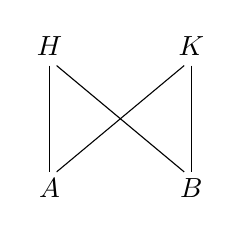
\begin{tikzpicture}[scale=0.9]
                \node [above] at (0,0) {$A$};
                \node [above] at (0,2) {$H$};
                \node [above] at (2,2) {$K$};
                \node [above] at (2,0) {$B$};
                \draw [-] (1.9,2) to (0.1,0.5);
                \draw [-] (2,2) to (2,0.5);
                \draw [-] (0,2) to (0,0.5);
                \draw [-] (0.1,2) to (1.9,0.5);
            \end{tikzpicture}
        \end{figure}
        But $A<H\cap K$, $B<H\cap K\Rightarrow A\vee B<H\cap K$. So $A\vee B\lhd H$, $A\vee B\lhd K$. That's contradictory! There is only one lower bound for $\{H,K\}$. Notice that $\{e\}<H\cap K$ so there exists at least one subgroup satisfies the condition. We have proved normality forms a lattice.
    \end{enumerate}
\end{answer}

$$ $$

\begin{ex}
    If $N_{1}\lhd G_{1}$, $N_{2}\lhd G_{2}$ then $(N_{1}\times N_{2})\lhd (G_{1}\times G_{2})$ and $(G_{1}\times G_{2})/(N_{1}\times N_{2})\cong (G_{1}/N_{1})\times(G_{2}/N_{2})$.
\end{ex}

\begin{answer}
    Take $a\in (N_{1}\times N_{2})$, $a=(n_{1},n_{2})$ where $n_{1}\in N_{1}$, $n_{2}\in N_{2}$. $\forall x\in (G_{1}\times G_{2})$, $x=(g_{1},g_{2})$ where $g_{1}\in G_{1}$, $g_{2}\in G_{2}$. $x^{-1}=(g_{1}^{-1},g_{2}^{-1})$, $x^{-1}ax=(g_{1}^{-1}n_{1}g_{1},g_{2}^{-1}n_{2}g_{2})$. $N_{1}\lhd G_{1}$, $N_{2}\lhd G_{2}$, so $g_{1}^{-1}n_{1}g_{1}\in N_{1}$, $g_{2}^{-1}n_{2}g_{2}\in N_{2}$. $x^{-1}ax\in (N_{1}\times N_{2})$. Thus $(N_{1}\times N_{2})\lhd (G_{1}\times G_{2})$.

    Assume $G_{1}=\bigcup\limits_{i\in I}N_{1}a_{i}$, $G_{2}=\bigcup\limits_{j\in J}N_{2}b_{j}$. Then $G_{1}\times G_{2}=\bigcup\limits_{i\in I}N_{1}a_{i}\times \bigcup\limits_{j\in J}N_{2}b_{j}$. Denote $A=\{a_{i}|i\in I\}$, $B=\{b_{j}|j\in J\}$. We construct two bijections $(G_{1}\times G_{2})/(N_{1}\times N_{2})\to A\times B$ and $(G_{1}/N_{1})\times(G_{2}/N_{2})$.\[f: N_{1}a_{i}\times N_{2}b_{j}\mapsto (a_{i},b_{j})\]\[g: (N_{1}a_{i}, N_{2}b_{j})\mapsto (a_{i},b_{j})\] Take $h=g^{-1}\circ f$, $f,g$ are bijections, so $h$ is an isomorphism. $(G_{1}\times G_{2})/(N_{1}\times N_{2})\cong (G_{1}/N_{1})\times(G_{2}/N_{2})$.
\end{answer}

$$ $$

\begin{ex}
    Let $N\lhd G$ and $K\lhd G$. If $N\cap K=\left\langle e\right\rangle$ and $N\vee K=G$, then $G/N\cong K$.
\end{ex}

\begin{answer}
    Assume $G=\bigcup\limits_{i\in I}Na_{i}$, we construct $f:k \to G /N$. We prove that $\forall x,y\in K$, $x,y$ belong to different cosets of $N$. Suppose not. $\exists x,y \in K$, $x,y\in Na_{i}$, then $xy^{-1}\in N\Rightarrow x=y$. That's contradictory! So $f$ is a monomorphism.

    $G=H\vee K$, so $G=HK$. we can write $x$ as $pq$, where $p\in H$, $q\in K$. $\left| G/H \right|=\left[G:H\right]=\left[HK:H\right]=\left[K:K\cap H\right]=\left| K \right| $. $f$ is a epimorphism.
    
    Thus, $G /N\cong K$.
\end{answer}

$$ $$

\begin{ex}
    If $f:G\to H$ is a homomorphism, $H$ is abelian and $N$ is a subgroup of $G$ containing $\mathrm{Ker}f$, then $N$ is normal in $G$.
\end{ex}

\begin{answer}
    Assume there exists $x\in G$, $x\notin N$ s.t. $f(x)\in f(N)$. $\exists n\in N$, $f(x)=f(n)$, $f(xn^{-1})=f(x)f(n)^{-1}=e'\Rightarrow xn^{-1}\in\mathrm{Ker}f\Rightarrow x\in N$. That's contradictory! $\forall x\in G$, $n\in N$, $f(x^{-1}nx)=f(x^{-1})f(n)f(x)=f(n)\in f(N)$, so $x^{-1}nx\in N$. Thus, $N\lhd G$.
\end{answer}

$$ $$

\begin{ex}
    \begin{enumerate}[(a)]
        \item Consider the subgroups $\left\langle 6\right\rangle$ and $\left\langle 30\right\rangle$ of $\mathbf{Z}$ and show that $\left\langle 6\right\rangle /\left\langle 30\right\rangle\cong Z_{5}$.
        \item For any $k,m>0$, $\left\langle k\right\rangle /\left\langle km\right\rangle\cong Z_{m}$; in particular, $\mathbf{Z}/\left\langle m\right\rangle=\left\langle 1\right\rangle /\left\langle m\right\rangle\cong Z_{m}$.
    \end{enumerate}
\end{ex}

\begin{answer}
    \begin{enumerate}[(a)]
        \item $\left\langle 6\right\rangle=\{6n|n\in \mathbf{Z}\}$, $\left\langle 30\right\rangle=\{30n|n\in \mathbf{Z}\}$. So $\left\langle 6\right\rangle/\left\langle 30\right\rangle=\{\left\langle 30\right\rangle, \left\langle 30\right\rangle +6, \left\langle 30\right\rangle +12, \left\langle 30\right\rangle +18, \left\langle 30\right\rangle +24\}\cong Z_{5}$
        \item $\left\langle km\right\rangle\lhd \left\langle k\right\rangle$, $\left\langle k\right\rangle=\bigcup\limits_{i\in I}(\left\langle km\right\rangle +a_{i})$. For $x\in \left\langle k\right\rangle$, $x\equiv a_{i}\mod km$, then $x\in \left\langle km \right\rangle +a_{i}$. $f:\left\langle k\right\rangle/\left\langle km\right\rangle\to \{a_{i}|i\in I\}$ defined by $f(\left\langle km\right\rangle +a_{i})=a_{i}$ is a bijection. We check that $g: \{a_{i}|i\in I\}\to Z_{m}$ is also a bijection. Define $b_{i}\equiv \frac{a_{i}}{k}\mod m$, $g(a_{i})=b_{i}$. If there exists $b_{i}=b_{j}$ for $i\neq j$, $a_{i}\equiv a_{j}\mod km$. That's contradictory! So $g$ is an injection. $g$ is obviously a surjection, so $g$ is a bijection. Take $h= g\circ f:\left\langle k\right\rangle /\left\langle km \right\rangle\to Z_{m}$ is a isomorphism, so $\left\langle k\right\rangle /\left\langle km \right\rangle\cong Z_{m}$.
    \end{enumerate}
\end{answer}

$$ $$

\begin{ex}
    If $f: G \to H$ is a homomorphism with kernel $N$ and $K<G$, then prove that $f^{-1}(f(K))=KN$. Hence $f^{-1}(f(K))=K$ if and only if $N<K$.
\end{ex}

\begin{answer}
    Take $x\in f^{-1}(f(K))$, then there exists $k\in K$ s.t. $f(x)=f(k)$. $f(xk^{-1})=f(x)f(k)^{-1}=e'\in f(K) \Rightarrow xk^{-1}\in\mathrm{Ker}f=N$. Thus, $x\in Nk\subset NK$, $f^{-1}(f(K))\subset NK$.

    $\forall x=nk\in NK$, where $n\in N$ and $k\in K$. $f(x)=f(n)f(k)=e'f(k)\in f(K)$, so $NK\subset f^{-1}(f(K))$.

    Thus, $f^{-1}(f(K))=NK$. Hence $f^{-1}(f(K))=K$ if and only if $N<K$.
\end{answer}

$$ $$

\begin{ex}
    If $N\lhd G$, $\left[G:H\right]$ finite, $H<G$, $\left| H \right| $ finite, and $\left[G:N\right]$ and $\left| H \right| $ are relatively prime, then $H<N$.
\end{ex}

\begin{answer}
    $N\lhd G\Rightarrow NH<G$. By the second isomorphism theorem, $NH /N\cong H/H\cap N\Rightarrow \left[NH:N\right]=\left[H:H\cap N\right]$. Assume $\left[G:N\right]=m$, $\left| H \right| =n$, $\left| G \right| =mnp$ where $(m,n)=1$. Then $\left| N \right| =np$, $N<NH$, assume $\left| NH \right| =knp$, $NH<G\Rightarrow knp|mnp\Rightarrow k|m$. $\left[NH:N\right]=\left[H:H\cap N\right]=k\Rightarrow k|n$. So $k=1$, $NH=N$ which means $H<N$.
\end{answer}

$$ $$

\begin{ex}
    If $N\lhd G$, $\left| N \right|$ finite, $H<G$, $\left[G:N\right] $ finite, and $\left[G:H\right]$ and $\left| N \right| $ are relatively prime, then $N<H$.
\end{ex}

\begin{answer}
    $N\lhd G\Rightarrow NH<G$. By the second isomorphism theorem, $NH /N\cong H/H\cap N\Rightarrow \left[NH:N\right]=\left[H:H\cap N\right]$. Assume $\left[G:H\right]=m$, $\left| N \right| =n$, $\left| G \right| =mnp$ where $(m,n)=1$. Then $\left| H \right| =np$, $H<NH$, assume $\left| NH \right| =knp$, $NH<G\Rightarrow knp|mnp\Rightarrow k|m$. $\left[NH:N\right]=\left[H:H\cap N\right]=kp\Rightarrow kp|np\Rightarrow k|n$. So $k=1$, $NH=H$ which means $N<H$.
\end{answer}

$$ $$

\begin{ex}
    If $H$ is a subgroup of $Z(p^{\infty})$ and $H\neq Z(p^{\infty})$, then $Z(p^{\infty}) /H\cong Z(p^{\infty})$.
\end{ex}

\begin{answer}
    From \textbf{Exercise 1.3.7}(b), we know that $H$ has the form $\left\langle \bar{\frac{1}{p^{n}}}\right\rangle$. Take $x_{i}=\bar{\frac{1}{p^{n+i}}}+H$, $x_{1}=\bar{\frac{1}{p^{n+1}}}+H$. \[\sum_{m=1}^{p}x_{1}=\bar{\frac{p}{p^{n+1}}}+pH=\bar{\frac{1}{p^{n}}}+H=H\] \[\sum_{m=1}^{p}x_{i}=\bar{\frac{p}{p^{n+i}}}+pH=\bar{\frac{1}{p^{n+i-1}}}+H=x_{i-1}\] Take $A=\{x_{i}|i\in \mathbf{Z}_{+}\}$, $\left\langle A\right\rangle\cong Z(p^{\infty})$ by \textbf{Exercise 1.3.7}(e). $\forall x\in \left\langle A\right\rangle$, $x\in Z(p^{\infty}) /H$, so $\left\langle A\right\rangle\subset Z(p^{\infty}) /H$. Take $x\in Z(p^{\infty}) /H$, $x=y+H$ where $y=\sum\limits_{i=1}^{m}\frac{a_{i}}{p^{n+i}}$, $x=\sum\limits_{i=1}^{m}(\frac{a_{i}}{p^{n+i}}+H)\in \left\langle A\right\rangle$. Thus, $Z(p^{\infty}) /H\subset \left\langle A\right\rangle$, $\left\langle A\right\rangle=Z(p^{\infty}) /H\cong Z(p^{\infty})$.
\end{answer}
\section{Symmetric, alternating, and dihedral groups}
\begin{ex}
    Find four different subgroups of $S_{4}$ that are isomorphic to $S_{3}$ and nine isomorphic to $S_{2}$.
\end{ex}

$$ $$

\begin{ex}
    \begin{enumerate}[(a)]
        \item $S_{n}$ is generated by the $n-1$ transpositions $(12)$, $(13)$, $(14)$, $\dots$, $(1n)$.
        \item $S_{n}$ is generated by the $n-1$ transpositions $(12), (23), (34),\dots, (n-1\, n)$.
    \end{enumerate}
\end{ex}

$$ $$

\begin{ex}
    If $\sigma=(i_{1}i_{2}\cdots i_{r})\in S_{n}$ and $\tau\in S_{n}$, then $\tau\sigma\tau^{-1}$ is the $r$-cycle $(\tau(i_{1})\tau(i_{2})\cdots\tau(i_{r}))$.
\end{ex}

$$ $$

\begin{ex}
    \begin{enumerate}[(a)]
    \item $S_{n}$  is generated by $\sigma_{1}=(12)$ and $\tau=(123\cdots n)$.
    \item $S_{n}$ is generated by $(12)$ and $(23\cdots n)$.
    \end{enumerate}
\end{ex}

$$ $$

\begin{ex}
    Let $\sigma, \tau \in S_{n}$. If $\sigma$ is even (odd), then so is $\tau\sigma\tau^{-1}$.
\end{ex}

$$ $$

\begin{ex}
    $A_{n}$ is the only subgroup of $S_{n}$ of index 2.
\end{ex}

$$ $$

\begin{ex}
    Show that $N=\{(1),(12)(34),(13)(24),(14)(23)\}$ is a normal subgroup of $S_{4}$ contained in $A_{4}$ such that $S_{4} /N\cong S_{3}$ and $A_{4} /N\cong Z_{3}$.
\end{ex}

$$ $$

\begin{ex}
    The group $A_{4}$ has no subgroup of order $6$.
\end{ex}

$$ $$

\begin{ex}
    For $n\geq 3$ let $G_{n}$ be the multiplicaive group of complex matrices generated by $x=\begin{pmatrix}
        0&1\\1&0
    \end{pmatrix}$ and $y=\begin{pmatrix}
        e^{2\pi i/n}&0\\0&e^{-2\pi i/n}
    \end{pmatrix}$, where $i^{2}=-1$. Show that $G_{n}\cong D_{n}$.
\end{ex}

$$ $$

\begin{ex}
    Let $a$ be the generator of order $n$ of $D_{n}$. Show that $\left\langle a\right\rangle\lhd D_{n}$ and $D_{n} /\left\langle a\right\rangle\cong Z_{2}$.
\end{ex}

$$ $$

\begin{ex}
    Find all normal subgroups of $D_{n}$.
\end{ex}

$$ $$

\begin{ex}
    The center of the group $D_{n}$ is $\left\langle e\right\rangle$ if $n$ is odd and isomorphic to $Z_{2}$ if $n$ is even.
\end{ex}

$$ $$

\begin{ex}
    For each $n\geq 3$ let $P_{n}$ be a regular polygon of $n$ sides (for $n=3$, $P_{n}$ is an equilateral triangle; for $n=4$, a square). A \emph{symmetry} of $P_{n}$ is a bijection $P_{n}\to P_{n}$ that preserves distances and maps adjacent vertices on to adjacent vertices.
    
    \begin{enumerate}[(a)]
        \item The set $D_{n}^{*}$ of all symmetries of $P_{n}$ is a group under the binary operation of composition of functions.
        \item Every $f\in D_{n}^{*}$ is completely determined by its actions on the vertices of $P_{n}$. Number the vertices consecutively $1,2,\dots, n$; then each $f\in D_{n}^{*}$ determines a unique permutation $\sigma_{f}$ of $\{1,2,\dots, n\}$. The assignment $f\mapsto \sigma_{f}$ defines a monomorphism of groups $\varphi:D_{n}^{*}\to S_{n}$.
        \item $D_{n}^{*}$ is generated by $f$ and $g$, where $f$ is a rotation of $2\pi /n$ degrees about the center of $P_{n}$ and $g$ is a reflection about the ``diameter'' through the center and vertex 1.
        \item $\sigma_{f}=(123\cdots n)$ and $\sigma_{g}=\begin{pmatrix}
            1&2&3&\cdots&n-1&n\\1&n&n-1&\cdots&3&2
        \end{pmatrix}$, whence \\$\mathrm{Im}\varphi=D_{n}$ and $D_{n}^{*}\cong D_{n}$.
    \end{enumerate}
\end{ex}
\section{Categories: products, coproducts, and free objects}
\begin{ex}
    A \emph{pointed set} is a pair $(S,x)$ with $S$ a set and $x\in S$. A morphism of pointed sets $(S,x)\to (S', x')$ is a triple $(f,x,x')$, where $S\to S'$ is a function such that $f(x)=x'$. Show that pointed sets form a category.
\end{ex}

\begin{answer}
    Let $\mathcal{S}$ be the category and 4 objects of $\mathcal{S}$ are $(A,a)$, $(B,b)$, $(C,c)$, $(D,d)$. $f$, $g$ and $h$ are morphisms defined by $f:A\to B$, $g:B\to C$, $h:C\to D$ with $f(a)=b$, $g(b)=c$, $h(c)=d$.

    \begin{figure}[H]\centering
        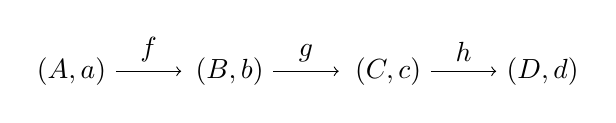
\begin{tikzpicture}
            \node [left] at (0,1) {$(A,a)$};
            \node [left] at (2,1) {$(B,b)$};
            \node [left] at (4,1) {$(C,c)$};
            \node [left] at (6,1) {$(D,d)$};
            \draw [->] (0,1)-- node [above, pos=0.5]{$f$}(0.83,1);
            \draw [->] (2,1)-- node [above, pos=0.5]{$g$}(2.83,1);
            \draw [->] (4,1)-- node [above, pos=0.5]{$h$}(4.83,1);
        \end{tikzpicture}
        \caption*{category $\mathcal{S}$}
    \end{figure}
    \[\mathrm{hom}(A,B)\times\mathrm{hom}(B,C)\to \mathrm{hom}(A,C)\]because $g\circ f:A\to C$ with $g(f(a))=g(b)=c=g\circ f(a)$. Similarly, $(h\circ g)\circ f=h\circ (g\circ f)$ with $(h\circ g)\circ f(a)=h\circ (g\circ f)(a)=d$. Take $1_{B}$ consist of those functions $i:B\to B$ with $i(b)=b$. Then $1_{B}\circ f=f$ and $g\circ 1_{B}=g$. So $\mathcal{S}$ is a category.
\end{answer}

$$ $$

\begin{ex}
    If $f:A\to B$ is an equivalence in a category $\mathcal{C}$ and $g:B\to A$ is the morphism such that $g\circ f=1_{A}$, $f\circ g=1_{B}$, show that $g$ is unique.
\end{ex}

\begin{answer}
    Assume there exist $g$ and $g'$ satisfies the condition.

    \begin{figure}[H]\centering
        \subfigure{
            \begin{minipage}[c]{0.3\linewidth}
                \centering
                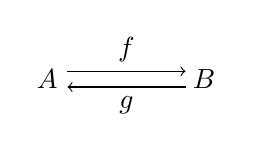
\begin{tikzpicture}
                    \node [left] at (0,1) {$A$};
                    \node [left] at (2,1) {$B$};
                    \draw [->] (0,1.1)-- node [above, pos=0.5]{$f$} (1.5,1.1);
                    \draw [<-] (0,0.9)-- node [below, pos=0.5]{$g$} (1.5,0.9);
                \end{tikzpicture}
            \end{minipage}
        }
        \subfigure{
            \begin{minipage}[c]{0.3\linewidth}
                \centering
                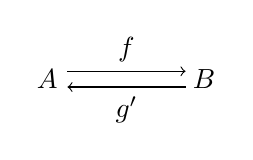
\begin{tikzpicture}
                    \node [left] at (0,1) {$A$};
                    \node [left] at (2,1) {$B$};
                    \draw [->] (0,1.1)-- node [above, pos=0.5]{$f$} (1.5,1.1);
                    \draw [<-] (0,0.9)-- node [below, pos=0.5]{$g'$} (1.5,0.9);
                \end{tikzpicture}
            \end{minipage}
        }
    \end{figure}
    So $g'\circ(f\circ g)=g'\circ 1_{B}=g'=(g'\circ f)\circ g=1_{A}\circ g =g$.
\end{answer}

$$ $$

\begin{ex}
    In the category $\mathcal{G}$ of groups, show that the group $G_{1}\times G_{2}$ together with the homomorphisms $\pi_{1}:G_{1}\times G_{2}\to G_{1}$ and $\pi_{2}:G_{1}\times G_{2}\to G_{2}$ is a product for $\{G_{1},G_{2}\}$.
\end{ex}

\begin{answer}
    Take $\tau_{1}:G_{1}\to G_{1}\times G_{2}$ as $\tau_{1}(g_{1})=(g_{1},e)$; $\tau_{2}:G_{2}\to G_{1}\times G_{2}$ as $\tau_{2}(g_{2})=(e,g_{2})$; $\pi_{1}:G_{1}\times G_{2}\to G_{1}$ as $\pi_{1}(g_{1},g_{2})=g_{1}$; $\pi_{2}:G_{1}\times G_{2}\to G_{2}$ as $\pi_{2}(g_{1},g_{2})=g_{2}$. Then

    \begin{figure}[H]\centering
        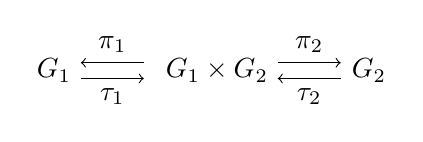
\begin{tikzpicture}
            \node [left] at (0,1) {$G_{1}$};
            \node [left] at (2.5,1) {$G_{1}\times G_{2}$};
            \node [left] at (4,1) {$G_{2}$};
            \draw [<-] (0,1.1)-- node [above, pos=0.5]{$\pi_{1}$} (0.8,1.1);
            \draw [->] (0,0.9)-- node [below, pos=0.5]{$\tau_{1}$} (0.8,0.9);
            \draw [->] (2.5,1.1)-- node [above, pos=0.5]{$\pi_{2}$} (3.3,1.1);
            \draw [<-] (2.5,0.9)-- node [below, pos=0.5]{$\tau_{2}$} (3.3,0.9);
        \end{tikzpicture}
    \end{figure}
    For any object $B$ such that

    \begin{figure}[H]\centering
        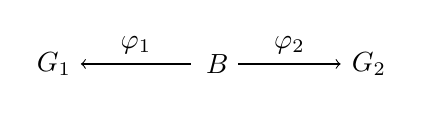
\begin{tikzpicture}
            \node [left] at (0,1) {$G_{1}$};
            \node [left] at (2,1) {$B$};
            \node [left] at (4,1) {$G_{2}$};
            \draw [<-] (0,1)-- node [above, pos=0.5]{$\varphi_{1}$} (1.4,1);
            \draw [->] (2,1)-- node [above, pos=0.5]{$\varphi_{2}$} (3.3,1);
        \end{tikzpicture}
    \end{figure}
    For any $x\in B$, define $f:B\to G_{1}\times G_{2}$ as $f(x)=(\varphi_{1}(x), \varphi_{2}(x))$. Then $\pi_{1}(f(x))=\varphi_{1}(x)$, $\pi_{1}\circ f=\varphi_{1}$, $\pi_{2}(f(x))=\varphi_{2}(x)$, $\pi_{2}\circ f=\varphi_{2}$. Thus
    
    \begin{figure}[H]\centering
        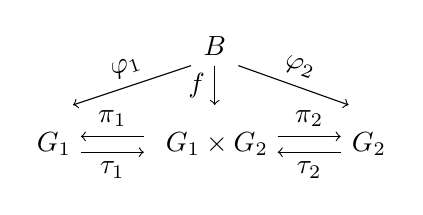
\begin{tikzpicture}
            \node [left] at (0,1) {$G_{1}$};
            \node [left] at (2.5,1) {$G_{1}\times G_{2}$};
            \node [left] at (4,1) {$G_{2}$};
            \draw [<-] (0,1.1)-- node [above, pos=0.5]{$\pi_{1}$} (0.8,1.1);
            \draw [->] (0,0.9)-- node [below, pos=0.5]{$\tau_{1}$} (0.8,0.9);
            \draw [->] (2.5,1.1)-- node [above, pos=0.5]{$\pi_{2}$} (3.3,1.1);
            \draw [<-] (2.5,0.9)-- node [below, pos=0.5]{$\tau_{2}$} (3.3,0.9);
            \node [above] at (1.7,2) {$B$};
            \draw [->] (1.7,2)-- node [left, pos=0.5]{$f$} (1.7,1.5);
            \draw [->] (1.4,2)-- node [above, pos=0.5, sloped]{$\varphi_{1}$} (-0.1,1.5);
            \draw [->] (2,2)-- node [above, pos=0.5, sloped]{$\varphi_{2}$} (3.4,1.5);
        \end{tikzpicture}
    \end{figure}
    Next we verify the uniqueness. If there exist $f$ and $f'$ satisfies the condition, \[\pi_{1}(f(x))=\pi_{1}(f'(x))=\varphi_{1}(x)\]\[\pi_{2}(f(x))=\pi_{2}(f'(x))=\varphi_{2}(x)\]Thus $f(x)=f'(x)$ for all $x\in B$, so $f=f'$.
\end{answer}

$$ $$

\begin{ex}
    In the category $\mathcal{A}$ of abelian groups, show that the group $A_{1}\times A_{2}$ together with the morphisms $\tau_{1}:A_{1}\to A_{1}\times A_{2}$ and $\tau_{2}:A_{2}\to A_{1}\times A_{2}$ is a coproduct of $\{A_{1}, A_{2}\}$.
\end{ex}

\begin{answer}
    Take $\tau_{1}:A_{1}\to A_{1}\times A_{2}$ as $\tau_{1}(a_{1})=(a_{1},e)$; $\tau_{2}:A_{2}\to A_{1}\times A_{2}$ as $\tau_{2}(a_{2})=(e,a_{2})$; $\pi_{1}:A_{1}\times A_{2}\to A_{1}$ as $\pi_{1}(a_{1},a_{2})=a_{1}$; $\pi_{2}:A_{1}\times A_{2}\to A_{2}$ as $\pi_{2}(a_{1},a_{2})=a_{2}$. Then

    \begin{figure}[H]\centering
        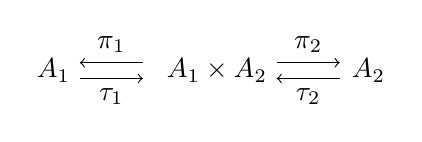
\begin{tikzpicture}
            \node [left] at (0,1) {$A_{1}$};
            \node [left] at (2.5,1) {$A_{1}\times A_{2}$};
            \node [left] at (4,1) {$A_{2}$};
            \draw [<-] (0,1.1)-- node [above, pos=0.5]{$\pi_{1}$} (0.8,1.1);
            \draw [->] (0,0.9)-- node [below, pos=0.5]{$\tau_{1}$} (0.8,0.9);
            \draw [->] (2.5,1.1)-- node [above, pos=0.5]{$\pi_{2}$} (3.3,1.1);
            \draw [<-] (2.5,0.9)-- node [below, pos=0.5]{$\tau_{2}$} (3.3,0.9);
        \end{tikzpicture}
    \end{figure}
    For any object $B$ such that

    \begin{figure}[H]\centering
        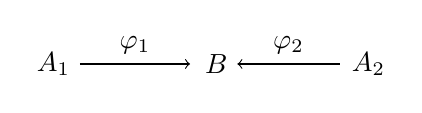
\begin{tikzpicture}
            \node [left] at (0,1) {$A_{1}$};
            \node [left] at (2,1) {$B$};
            \node [left] at (4,1) {$A_{2}$};
            \draw [->] (0,1)-- node [above, pos=0.5]{$\varphi_{1}$} (1.4,1);
            \draw [<-] (2,1)-- node [above, pos=0.5]{$\varphi_{2}$} (3.3,1);
        \end{tikzpicture}
    \end{figure}
    For any $(a_{1},a_{2})\in A_{1}\times A_{2}$, define $f:A_{1}\times A_{2}\to B$ as $f(a_{1},a_{2})=\varphi_{1}(a_{1})\varphi_{2}(a_{2})$. Then $f(\tau_{1}(a_{1}))=f(a_{1},e)=\varphi_{1}(a_{1})e=\varphi_{1}(a_{1})$, $f\circ \tau_{1}=\varphi_{1}$, $f(\tau_{2}(a_{2}))=f(e,a_{2})=e\varphi_{2}(a_{2})=\varphi_{2}(a_{2})$, $f\circ \tau_{2}=\varphi_{2}$.

    \begin{figure}[H]\centering
        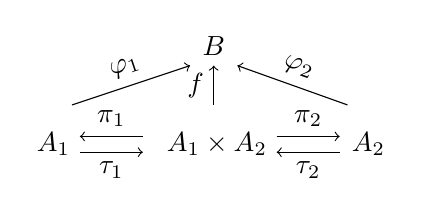
\begin{tikzpicture}
            \node [left] at (0,1) {$A_{1}$};
            \node [left] at (2.5,1) {$A_{1}\times A_{2}$};
            \node [left] at (4,1) {$A_{2}$};
            \draw [<-] (0,1.1)-- node [above, pos=0.5]{$\pi_{1}$} (0.8,1.1);
            \draw [->] (0,0.9)-- node [below, pos=0.5]{$\tau_{1}$} (0.8,0.9);
            \draw [->] (2.5,1.1)-- node [above, pos=0.5]{$\pi_{2}$} (3.3,1.1);
            \draw [<-] (2.5,0.9)-- node [below, pos=0.5]{$\tau_{2}$} (3.3,0.9);
            \node [above] at (1.7,2) {$B$};
            \draw [<-] (1.7,2)-- node [left, pos=0.5]{$f$} (1.7,1.5);
            \draw [<-] (1.4,2)-- node [above, pos=0.5, sloped]{$\varphi_{1}$} (-0.1,1.5);
            \draw [<-] (2,2)-- node [above, pos=0.5, sloped]{$\varphi_{2}$} (3.4,1.5);
        \end{tikzpicture}
    \end{figure}
    Next we verify the uniqueness. If there exist $f$ and $f'$ satisfies the condition, \[f(\tau_{1}(a_{1}))=f'(\tau_{1}(a_{1}))=f(a_{1},e)=f'(a_{1},e)\]\[f(\tau_{2}(a_{2}))=f'(\tau_{2}(a_{2}))=f(e,a_{2})=f'(e,a_{2})\]\[\begin{aligned}
        &f(\tau_{1}(a_{1}),\tau_{2}(a_{2}))=f(\tau_{1}(a_{1}))f(\tau_{2}(a_{2}))\\=&f'(\tau_{1}(a_{1}),\tau_{2}(a_{2}))=f'(\tau_{1}(a_{1}))f'(\tau_{2}(a_{2}))
    \end{aligned}\]
    so $f=f'$.
\end{answer}

$$ $$

\begin{ex}
    Every family $\{A_{i}|i\in I\}$ in the category of sets has a coproduct.
\end{ex}

\begin{answer}
    We examine $\bigcup\limits^{\cdot}A_{i}=\{(a,i)\in (\cup A_{i})\times I|a\in A_{i}\}$ which satisfies the condition. Define the morphism $\pi_{i}:A_{i}\to \bigcup\limits^{\cdot}A_{i}$ as $\pi_{i}(a)=(a,i)$. For any $B$ such that $\exists \varphi_{i}:A_{i}\to B$.
    
    \begin{figure}[H]\centering
        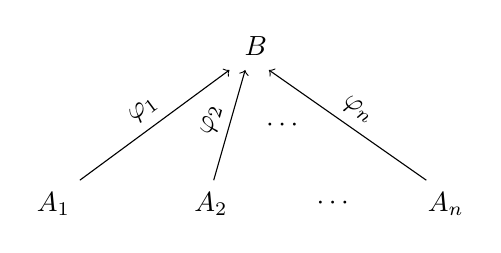
\begin{tikzpicture}
            \node [left] at (0,1) {$A_{1}$};
            \node [left] at (2,1) {$A_{2}$};
            \node [left] at (3.6,1) {$\cdots$};
            \node [left] at (5,1) {$A_{n}$};
            \node [left] at (2.5,3) {$B$};
            \draw [->] (0,1.3)-- node [above, pos=0.5, sloped]{$\varphi_{1}$} (1.9,2.7);
            \draw [->] (1.7,1.3)-- node [above, pos=0.5, sloped]{$\varphi_{2}$} (2.1,2.7);
            \draw [->] (4.4,1.3)-- node [above, pos=0.5, sloped]{$\varphi_{n}$} (2.4,2.7);
            \node [above] at (2.6,1.8) {$\cdots$};
        \end{tikzpicture}
    \end{figure}
    $\varphi(a)=x\in B$. Take $\varphi(a,i)=\varphi_{i}(a)$ defined on the subset of $\cup A_{i}\times I$, we can verify that the domain of $\varphi$ is $\bigcup\limits^{\cdot}A_{i}$. Then take $f=\varphi$, $f(\pi_{i}(a))=\varphi_{i}(a)$, $f\circ \pi_{i}=\varphi_{i}$.

    The uniqueness is obvious.
\end{answer}

$$ $$

\begin{ex}
    \begin{enumerate}[(a)]
        \item Show that in the category $\mathcal{S}_{*}$ of pointed sets product always exist; describe them.
        \item Show that in $\mathcal{S}_{*}$ every family of objects has a coproduct, describe the coproduct.
    \end{enumerate}
\end{ex}

\begin{answer}
    \begin{enumerate}[(a)]
        \item Define $\otimes$ as an operator between points and other elements in the pointed set. $\forall a\in A_{i}$, $a\otimes a_{i}=a_{1}\times a=a$. For a family of sets with their points $\{(A_{i},a_{i}|i\in I)\}$, consider $(A_{1}, A_{2}, \cdots, A_{n})=\{(a_{1}', a_{2}',\cdots, a_{n}')\}$. Define morphisms $\pi_{i}(a)=(a_{1}, a_{2},\cdots, a,\cdots, a_{n})$, $\pi_{i}:A_{i}\to (A_{1}, A_{2}, \cdots, A_{n})$.
        
        \begin{figure}[H]\centering
            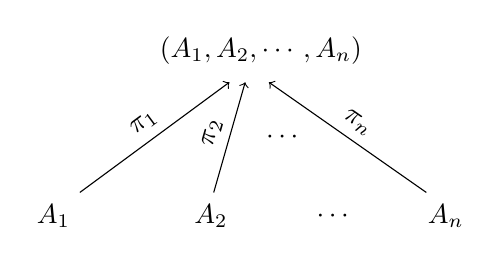
\begin{tikzpicture}
                \node [left] at (0,1) {$A_{1}$};
                \node [left] at (2,1) {$A_{2}$};
                \node [left] at (3.6,1) {$\cdots$};
                \node [left] at (5,1) {$A_{n}$};
                \node [above] at (2.3,2.8) {$(A_{1}, A_{2}, \cdots, A_{n})$};
                \draw [->] (0,1.3)-- node [above, pos=0.5, sloped]{$\pi_{1}$} (1.9,2.7);
                \draw [->] (1.7,1.3)-- node [above, pos=0.5, sloped]{$\pi_{2}$} (2.1,2.7);
                \draw [->] (4.4,1.3)-- node [above, pos=0.5, sloped]{$\pi_{n}$} (2.4,2.7);
                \node [above] at (2.6,1.8) {$\cdots$};
            \end{tikzpicture}
        \end{figure}
        For any $B$ such that $\exists \varphi_{i}:A_{i}\to B$.
    
        \begin{figure}[H]\centering
            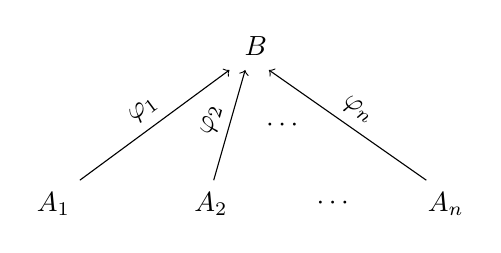
\begin{tikzpicture}
                \node [left] at (0,1) {$A_{1}$};
                \node [left] at (2,1) {$A_{2}$};
                \node [left] at (3.6,1) {$\cdots$};
                \node [left] at (5,1) {$A_{n}$};
                \node [left] at (2.5,3) {$B$};
                \draw [->] (0,1.3)-- node [above, pos=0.5, sloped]{$\varphi_{1}$} (1.9,2.7);
                \draw [->] (1.7,1.3)-- node [above, pos=0.5, sloped]{$\varphi_{2}$} (2.1,2.7);
                \draw [->] (4.4,1.3)-- node [above, pos=0.5, sloped]{$\varphi_{n}$} (2.4,2.7);
                \node [above] at (2.6,1.8) {$\cdots$};
            \end{tikzpicture}
        \end{figure}
        Take $f:(A_{1}, A_{2}, \cdots, A_{n})\to B$ as \[f(a_{1}',a_{2}',\cdots,a_{n}')=\varphi_{1}(a_{1}')\otimes\varphi_{2}(a_{2}')\otimes\cdots\otimes\varphi(a_{n}')\]Then $f\circ\pi_{i}(a)=f(a_{1},a_{2},\cdots,a,\cdots, a_{n})=\varphi_{1}(a_{1})\otimes\cdots\otimes\varphi_{i}(a)\otimes\cdots\otimes\varphi_{n}(a_{n})=\varphi_{i}(a)$. So $f\circ \pi_{i}=\varphi_{i}$.

        Next we verify the uniqueness. If there exist $f$ and $f'$ satisfies the condition. Then $\exists i\in I$ and $a\in A_{i}$ s.t. $f(a_{1},a_{2},\cdots,a,\cdots,a_{n})\neq f'(a_{1},a_{2},\cdots,a,\cdots,a_{n})$. But $f(\pi_{i}(a))=f'(\pi_{i}(a))$, so $f=f'$.
        \item The proof is similar to \textbf{Exercise 1.7.5}.
    \end{enumerate}
\end{answer}

$$ $$

\begin{ex}
    Let $F$ be a free object on a set $X(i:X\to F)$ in a concrete category $\mathcal{C}$. If $\mathcal{C}$ contains an object whose underlying set has at least two elements in it, then $i$ is an injective map of sets.
\end{ex}

\begin{answer}
    Assume $A\in\mathrm{obj}(\mathcal{C})$, $A$ has at least two elements and $X\xrightarrow{f} A$. $X\xrightarrow{i} F$ and $F$ is free on $X$, so there exists a morphism $\bar{f}$ s.t. $F\xrightarrow{\bar{f}}A$. If $\left| X \right|=1$, $i$ must be injective. For $\left| X \right| \geq 2$. Suppose $i$ is not injective. Take $x_{1}, x_{2}\in X$ and $i(x_{1})=i(x_{2})\in F$, $f(x_{1})=a_{1}$, $f(x_{2})=a_{2}$. $\bar{f}(i(x_{1}))=\bar{f}(i(x_{2}))=f(x_{1})=f(x_{2})=a_{1}=a_{2}$. That means all the elements in $A$ are identical. That's contradictory to the assumption.
\end{answer}

$$ $$

\begin{ex}
    Suppose $X$ is a set and $F$ is a free object on $X$ (with $i:X\to F$) in the category of groups. Prove that $i(X)$ is a set of generators for the group $F$.
\end{ex}

\begin{answer}
    Assume $G$ the subgroup of $F$ is the group generated by $i(X)$. Since $X\xrightarrow{i}G$ and $X\xrightarrow{i}F$, we can obtain unique morphism $\varphi$ such that $F\xrightarrow{\varphi}G$ and $\varphi \circ i=i$. 
    
    Consider morphism $1_{F}:F\to F$ which is the identical homomorphism. $F$ is free so $1_{F}$ is the unique homomorphism. Take $\subset:G\to F$ as a morphism defined as $\forall g\in G$, $\subset(g)=g$. Then
    
    \begin{figure}[H]\centering
        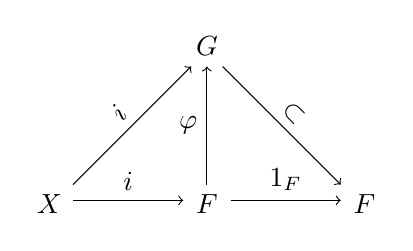
\begin{tikzpicture}
        \node [below] at (0,1) {$X$};
        \node [below] at (2,1) {$F$};
        \node [below] at (4,1) {$F$};
        \node [below] at (2,3) {$G$};
        \draw [->] (0.3,0.8)-- node [above, pos=0.5] {$i$} (1.7,0.8);
        \draw [->] (2.3,0.8)-- node [above, pos=0.5] {$1_{F}$} (3.7,0.8);
        \draw [->] (2,1)-- node [left, pos=0.5] {$\varphi$} (2,2.5);
        \draw [->] (0.3,1)-- node [above, pos=0.5, sloped] {$i$} (1.8,2.5);
        \draw [<-] (3.7,1)-- node [above, pos=0.5, sloped] {$\subset$} (2.2,2.5);
        \end{tikzpicture}
    \end{figure}
    $\subset\circ\varphi\circ i=1_{F}\circ i=i$ so $\subset\circ\varphi=1_{F}$. Thus $\subset$ is an epimorphism, $F\subset G$. So $F=G$ can be generated by $i(X)$.
\end{answer}
\section{Direct products and direct sums}
\begin{ex}
    $S_{3}$ is not the direct product of any family of its proper subgroups. The same is true of $Z_{p^{n}}$($p$ prime, $n\geq 1$) and $\mathbb{Z}$.
\end{ex}

\begin{answer}
    We list all the subgroups of $S_{3}$: $\{(1), (12)\}$, $\{(1), (13)\}$, $\{(1), (23)\}$, $\{(1), (123), (132)\}$. Only $\{(1), (123), (132)\}$ is normal, so $S_{3}$ isn't an direct product of any family of its proper subgroups.

    For $Z_{p^{n}}$, $Z_{p^{i}}\lhd Z_{p^{n}}$ for all $i=1,2,\dots ,n-1$ but $Z_{p^{i}}\cap Z_{p^{j}}\neq \{e\}$. So $Z_{p^{n}}$ isn't an direct product of any family of its proper subgroups.

    For $\mathbf{Z}$. $\forall N_{1}\lhd \mathbf{Z}$, $N_{2}\lhd \mathbf{Z}$, we have $N_{1}=\left\langle a_{1}\right\rangle$ and $N_{2}=\left\langle a_{2}\right\rangle$. Thus, $N_{1}\cap N_{2}=\left\langle a_{1}a_{2}\right\rangle\neq \{e\}$. So $\mathbf{Z}$ isn't an direct product of any family of its proper subgroups.
\end{answer}

$$ $$

\begin{ex}
    Give an example of groups $H_{i}$, $K_{i}$ such that $H_{1}\times H_{2}\cong K_{1}\times K_{2}$ and no $H_{i}$ is isomorphic to any $K_{j}$.
\end{ex}

\begin{answer}
    Take $H_{1}\cong K_{1}\times K_{2}$, $H_{2}=\{e\}$. We verify that $H_{1}\times H_{2}\cong K_{1}\times K_{2}$. There exists $f:H_{1}\to K_{1}\times H_{2}$ which is an isomorphism. There exists canonical projection $\pi_{1}:H_{1}\times H_{2}\to H_{1}$ and $\pi_{1}$ is an epimorphism. $\mathrm{Ker}\pi_{1}=\{(e_{1},e_{2})\}$ thus $\pi_{1}$ is also a monomorphism. Therefore $\bar{f}=f\circ \pi_{1}$ is a well defined isomorphism. $H_{1}\times H_{2}\cong K_{1}\times K_{2}$ but neither $H_{1}$ nor $H_{2}$ are isomorphic to any $K_{i}$, $i=1,2$.
\end{answer}

$$ $$

\begin{ex}
    Let $G$ be and (additive) abelian group with subgroups $H$ and $K$. Show that $G\cong H\oplus K$ if and only if there are homomorphisms 
    
    \begin{figure}[H]\centering
        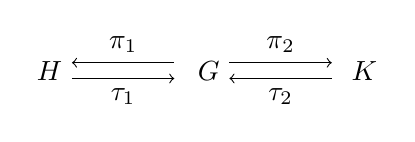
\begin{tikzpicture}
            \node [left] at (0,1) {$H$};
            \node [left] at (2,1) {$G$};
            \node [left] at (4,1) {$K$};
            \draw [<-] (0,1.1)-- node [above, pos=0.5]{$\pi_{1}$} (1.3,1.1);
            \draw [->] (0,0.9)-- node [below, pos=0.5]{$\tau_{1}$} (1.3,0.9);
            \draw [->] (2,1.1)-- node [above, pos=0.5]{$\pi_{2}$} (3.3,1.1);
            \draw [<-] (2,0.9)-- node [below, pos=0.5]{$\tau_{2}$} (3.3,0.9);
        \end{tikzpicture}
    \end{figure}
    such that $\pi_{1}\tau_{1}=1_{H}$, $\pi_{2}\tau_{2}=1_{K}$, $\pi_{1}\tau_{2}=0$ and $\pi_{2}\tau_{1}=0$, where 0 is the map sending every element onto the zero (identity) element, and $\tau_{1}\pi_{1}(x)+\tau_{2}\pi_{2}(x)=x$ for all $x\in G$.
\end{ex}

\begin{answer}
    If $G\cong H\oplus K$. Denote $f:G\to H\oplus K$ which is a isomorphism. Then there are canonical products $\pi_{1}'$, $\pi_{2}'$, $\tau_{1}'$, $\tau_{2}'$. 

    \begin{figure}[H]\centering
        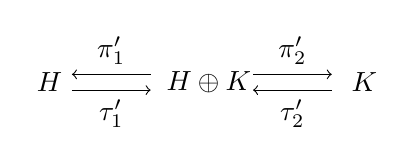
\begin{tikzpicture}
            \node [left] at (0,1) {$H$};
            \node [left] at (2.4,1) {$H\oplus K$};
            \node [left] at (4,1) {$K$};
            \draw [<-] (0,1.1)-- node [above, pos=0.5]{$\pi_{1}'$} (1,1.1);
            \draw [->] (0,0.9)-- node [below, pos=0.5]{$\tau_{1}'$} (1,0.9);
            \draw [->] (2.3,1.1)-- node [above, pos=0.5]{$\pi_{2}'$} (3.3,1.1);
            \draw [<-] (2.3,0.9)-- node [below, pos=0.5]{$\tau_{2}'$} (3.3,0.9);
        \end{tikzpicture}
    \end{figure}
    Thus

    \begin{figure}[H]\centering
        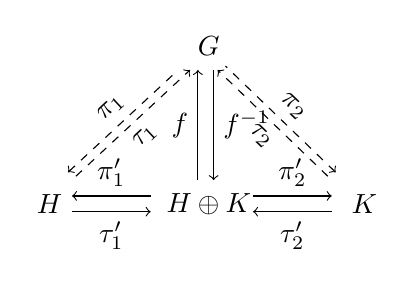
\begin{tikzpicture}
            \node [left] at (0,1) {$H$};
            \node [left] at (2.4,1) {$H\oplus K$};
            \node [left] at (4,1) {$K$};
            \node [left] at (2,3) {$G$};
            \draw [<-] (0,1.1)-- node [above, pos=0.5]{$\pi_{1}'$} (1,1.1);
            \draw [->] (0,0.9)-- node [below, pos=0.5]{$\tau_{1}'$} (1,0.9);
            \draw [->] (2.3,1.1)-- node [above, pos=0.5]{$\pi_{2}'$} (3.3,1.1);
            \draw [<-] (2.3,0.9)-- node [below, pos=0.5]{$\tau_{2}'$} (3.3,0.9);
            \draw [->] (1.6,1.3)-- node [left, pos=0.5]{$f$} (1.6,2.7);
            \draw [<-] (1.8,1.3)-- node [right, pos=0.5]{$f^{-1}$} (1.8,2.7);
            \draw [<-, dashed] (-0.05,1.4)-- node [above, pos=0.5, sloped]{$\pi_{1}$} (1.35,2.7);
            \draw [->, dashed] (0.05,1.35)-- node [below, pos=0.5, sloped]{$\tau_{1}$} (1.5,2.7);
            \draw [<-, dashed] (3.35,1.4)-- node [above, pos=0.5, sloped]{$\pi_{2}$} (1.95,2.75);
            \draw [->, dashed] (3.25,1.35)-- node [below, pos=0.5, sloped]{$\tau_{2}$} (1.85,2.7);
        \end{tikzpicture}
    \end{figure}
    Take $\tau_{1}=f\circ \tau_{1}'$, $\tau_{2}=f\circ \tau_{2}'$, $\pi_{1}=\pi_{1}'\circ f^{-1}$, $\pi_{2}=\pi_{2}'\circ f^{-1}$.
    \[\pi_{1}\tau_{1}=\pi_{1}'f^{-1}f\tau_{1}'=\pi_{1}'\tau_{1}'=1_{H}\]
    \[\pi_{2}\tau_{2}=\pi_{2}'f^{-1}f\tau_{2}'=\pi_{2}'\tau_{2}'=1_{K}\]
    \[\pi_{1}\tau_{2}=\pi_{1}'f^{-1}f\tau_{2}'=\pi_{1}'\tau_{2}'=0\]
    \[\pi_{2}\tau_{1}=\pi_{2}'f^{-1}f\tau_{1}'=\pi_{2}'\tau_{1}'=0\]
    $\forall x\in G$, $x=hk$ where $h\in H$ and $k\in K$. \[\begin{aligned}
        \tau_{1}\pi_{1}(x)+\tau_{2}\pi_{2}(x)&=f(\tau_{1}'\pi_{1}'(h,k))+f(\tau_{2}'\pi_{2}(h,k))\\&=f(\tau_{1}'(h))+f(\tau_{2}'(k))\\&=f(h,e)+f(e,k)\\&=f(h+e,e+k)=f(h,k)\\&=x
    \end{aligned}\]

    If there exist $\pi_{1}$, $\pi_{2}$, $\tau_{1}$, $\tau_{2}$ satisfies the condition. There are canonical projections $\pi_{1}'$, $\pi_{2}'$, $\tau_{1}'$, $\tau_{2}'$ between $H$ and $H\oplus K$, $K$ and $H\oplus K$.

    \begin{figure}[H]\centering
        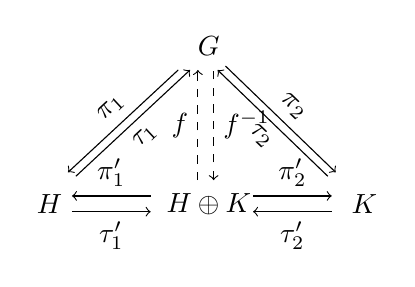
\begin{tikzpicture}
            \node [left] at (0,1) {$H$};
            \node [left] at (2.4,1) {$H\oplus K$};
            \node [left] at (4,1) {$K$};
            \node [left] at (2,3) {$G$};
            \draw [<-] (0,1.1)-- node [above, pos=0.5]{$\pi_{1}'$} (1,1.1);
            \draw [->] (0,0.9)-- node [below, pos=0.5]{$\tau_{1}'$} (1,0.9);
            \draw [->] (2.3,1.1)-- node [above, pos=0.5]{$\pi_{2}'$} (3.3,1.1);
            \draw [<-] (2.3,0.9)-- node [below, pos=0.5]{$\tau_{2}'$} (3.3,0.9);
            \draw [->, dashed] (1.6,1.3)-- node [left, pos=0.5]{$f$} (1.6,2.7);
            \draw [<-, dashed] (1.8,1.3)-- node [right, pos=0.5]{$f^{-1}$} (1.8,2.7);
            \draw [<-] (-0.05,1.4)-- node [above, pos=0.5, sloped]{$\pi_{1}$} (1.35,2.7);
            \draw [->] (0.05,1.35)-- node [below, pos=0.5, sloped]{$\tau_{1}$} (1.5,2.7);
            \draw [<-] (3.35,1.4)-- node [above, pos=0.5, sloped]{$\pi_{2}$} (1.95,2.75);
            \draw [->] (3.25,1.35)-- node [below, pos=0.5, sloped]{$\tau_{2}$} (1.85,2.7);
        \end{tikzpicture}
    \end{figure}
    For $f=\tau_{1}'\pi_{1}+\tau_{2}'\pi_{2}$ which is a well defined homomorphism. $\forall h\in H$ and $k\in K$, $\tau_{1}'(h)+\tau_{2}'(k)=(h,k)\in H\oplus K$. Thus $f(x)=(e_{1},e_{2})$ if and only if $\pi_{1}(x)=e_{1}$ and $\pi_{2}(x)=e_{2}$. $\tau_{1}\pi_{1}(x)+\tau_{2}\pi_{2}(x)=\tau_{1}(e_{1})+\tau_{2}(e_{2})=e=x$. Thus $\mathrm{Ker}f=\{e\}$. $f$ is a monomorphism. $\forall (h,k)\in H\oplus K$, take $x=\tau_{1}(h)+\tau_{2}(k)\in G$, then \[\begin{aligned}
        f(x)&=\tau_{1}'\pi_{1}\tau_{1}(h)+\tau_1'\pi_{1}\tau_{2}(h)+\tau_{2}'\pi_{2}\tau_{1}(k)+\tau_{2}'\pi_{2}\tau_{1}(k)\\&=\tau_{1}'(h)+\tau_{2}'(k)=(h,k)\in H\oplus K
    \end{aligned}\]
    $f$ is a epimorphism. Thus $G\cong H\oplus K$.
\end{answer}

$$ $$

\begin{ex}
    Give an example to show that the weak direct product is not a coproduct in the category of all groups.
\end{ex}

\begin{answer}
    Consider $S_{3}$ and $S_{3}\times S_{3}$.

    \begin{figure}[H]\centering
        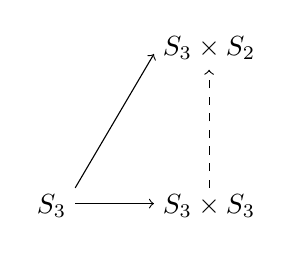
\begin{tikzpicture}
            \node [above] at (0,0) {$S_{3}$};
            \node [above] at (2,0) {$S_{3}\times S_{3}$};
            \node [above] at (2,2) {$S_{3}\times S_{2}$};
            \draw [->] (0.3,0.3) to (1.3,0.3);
            \draw [->] (0.3,0.5) to (1.3,2.2);
            \draw [->, dashed] (2,0.5) to (2,2);
        \end{tikzpicture}
    \end{figure}
    Since there doesn't exist homomorphism $S_{3}\to S_{2}$, there is no homomorphism $S_{3}\times S_{3}\to S_{3}\times S_{2}$.
\end{answer}

$$ $$

\begin{ex}
    Let $G$, $H$ be finite cyclic groups. Then $G\times H$ is cyclic if and only if $(\left| G \right|, \left| H \right|  )=1$.
\end{ex}

\begin{answer}
    Assume $\left| G \right| =m$, $\left| H \right| =n$, then $G\cong Z_{m}$, $H\cong Z_{n}$ and $G\times H\cong Z_{m}\oplus Z_{n}$.
    
    If$(\left| G \right| ,\left| H \right| )=1$. Consider $(x_{1}, x_{2})\in Z_{m}\oplus Z_{n}$. By \emph{Chinese Remainder Theorem}, there exists $x$ such that $a\equiv x\mod \mathrm{lcm}(m,n)$ and $a\equiv x_{1}\mod m$, $a\equiv x_{2}\mod n$. Thus, $a(1,1)=(x_{1},x_{2})$. $Z_{m}\oplus Z_{n}<\left\langle (1,1)\right\rangle$. $\left\langle (1,1)\right\rangle<Z_{m}\oplus Z_{n}$ is trivial. So $Z_{m}\oplus Z_{n}=\left\langle(1,1)\right\rangle\cong G\times H$ is cyclic.

    If $G\times H$ is cyclic. Assume $l=\gcd(m,n)$ and there exist $x$ such that  $x_{1}\equiv x\mod m$, $x_{2}\equiv x\mod n$. Take $x_{1}\not\equiv x_{2}\mod l$, it can be chosen properly. Consider $(x_{1}, x_{2})\in Z_{m}\oplus Z_{n}$, $x=k_{1}m+x_{1}=k_{2}n+x_{2}\Rightarrow x_{1}\equiv x_{2}\mod l$. That's contradictory!
\end{answer}

$$ $$

\begin{ex}
    Every finitely generated abelian group $G\neq\left\langle e\right\rangle$ in which every element (except $e$) has order $p$ ($p$ prime) is isomorphic to $Z_{p}\oplus Z_{p}\oplus\cdots\oplus Z_{p}$($n$ summands) for some $n\geq 1$.
\end{ex}

\begin{answer}
    Assume $\{a_{1}, a_{2}, \dots, a_{n}\}$ generates $G$. $\left| a_{i} \right| =p$ for $i=1,2,\dots, n$  so $\left\langle a_{i}\right\rangle\cong Z_{p}$. Now we show that $G=\prod\limits_{i=1}^{n}{^{w}}\left\langle a_{i}\right\rangle\cong \sum\limits_{i=1}^{n}Z_{p}$. $G=\left\langle a_{1}, a_{2},\dots, a_{n}\right\rangle$ and $\left\langle a_{1}\right\rangle\lhd G$ for $i=1,2,\dots, n$. If exist $\left\langle a_{i}\right\rangle$ s.t. $\prod\limits_{j=1, j\neq i}^{n}\left\langle a_{j}\right\rangle\cap \left\langle a_{i}\right\rangle\neq \{e\}$. Then there exists $a_{i}^{s_{i}}=a_{1}^{s_{1}}\cdots a_{i-1}^{s_{i-1}}a_{i+1}^{s_{i+1}}\cdots a_{n}^{s_{n}}$. $(s_{i},p)=1$ so $\exists 1\leq t_{i}\leq p-1$ such that $s_{i}t_{i}\equiv 1\mod p$. So $a_{i}^{s_{i}t_{i}}=a_{1}^{s_{1}t_{i}}\cdots a_{i-1}^{s_{i-1}t_{i}}a_{i+1}^{s_{i+1}t_{i}}\cdots a_{n}^{s_{n}t_{i}}=a_{i}$. $\{a_{1}, a_{2}, \dots, a_{n}\}$ can generate $G$. That's contradictory! So $\prod\limits_{j=1, j\neq i}^{n}\left\langle a_{j}\right\rangle\cap \left\langle a_{i}\right\rangle=\{e\}$, which means $G=\prod\limits_{i=1}^{n}{^{w}}\left\langle a_{i}\right\rangle\cong \sum\limits_{i=1}^{n}Z_{p}$.
\end{answer}

$$ $$

\begin{ex}
    Let $H,K,N$ be nontrivial normal subgroups of a group $G$ and suppose $G=H\times K$. Prove that $N$ is in the center of $G$ or $N$ intersects one of $H,K$ nontrivially. Give examples to show that both possibilities can actually occur when $G$ is nonabelian.
\end{ex}

\begin{answer}
    If $N\cap H=N\cap K=\{e\}$. $G=HK$. $\forall h\in H$ and $k\in K$, since $H\cap K=\{e\}$, $hk=kh$. For any $hk\in N$, and $h_{1}\in H\subset HK$, $h_{1}^{-1}hkh_{1}=h_{1}^{-1}hh_{1}k\in N$. Assume $h'=h_{1}^{-1}h_{1}\in H$, $h'k\in N$. Thus $h'^{-1}k^{-1}kh=h'^{-1}h\in N$. So $h'^{-1}h=e$, $h=h'$, $h$ is in the center $C(H)$ of group $H$. Similarly, $k\in C(K)$ which is the center of $K$. Then $\forall hk\in N$ and $h_{1}k_{1}\in G$, $k_{1}^{-1}h_{1}^{-1}hkh_{1}k_{1}=h_{1}^{-1}hh_{1}k_{1}^{-1}kk_{1}=hk$. $N\subset N(G)$.

    For $N\cup H\neq \varnothing$, the example can be trivial: $N<H$ and $N\lhd G$. There's many cyclic group satisfy the condition.

    For $N\subset C(G)$. Take $G=D_{4}^{*}\times D_{4}^{*}$, $H=D_{4}^{*}\times \{I\}$, $K=\{I\}\times D_{4}^{*}$. $\{I,R^{2}\}$ is normal in $D_{4}^{*}$. Denote $N$ is the subgroup $\{(I,I), (R^{2},R^{2})\}$. We can verify that $N$ satisfies the condition.
\end{answer}

$$ $$

\begin{ex}
    Corollary 8.7 is false if one of the $N_{i}$ is not normal.
\end{ex}

\begin{answer}
    Consider $N_{1}, N_{2},\dots , N_{n}$ are all finite. WLOG, assume $N_{1}$ is not normal. $G=\left\langle\bigcup\limits_{i=1}^{n}N_{i}\cup N_{1}\right\rangle$ and $N_{1}N_{2}\cdots N_{n}\subset G$. Denote $A=N_{2}N_{3}\cdots N_{n}$. Then $\exists a\in A$ such that $a^{-1}na=n'\notin N_{1}$. Thus $n'a\in G$ but $n'a\notin N_{1}N_{2}\cdots N_{n}$ so $\left| G \right| >\left| N_{1}N_{2}\cdots N_{n} \right| =\left| N_{1} \right|\times\left| N_{2} \right|\times\cdots\times\left| N_{n} \right| =\left| N_{1}\times N_{2}\times\cdots\times N_{n} \right| $.
\end{answer}

$$ $$

\begin{ex}
    If a group $G$ is the (internal) direct product of its subgroups $H$, $K$, then $H\cong G / K$ and $G /H \cong K$.
\end{ex}

\begin{answer}
    $H\cap K=\{e\}$. $G=H\times K=HK$. Thus $HK / H\cong K/(K\cap H)=K$, $HK /K\cong H /(K\cap H)=H$.
\end{answer}

$$ $$

\begin{ex}
    If $\{G_{i}|i\in I\}$ is a family of groups, then $\prod^{w}G_{i}$ is the internal weak product its subgroups $\{\tau_{i}(G_{i})|i\in I\}$.
\end{ex}

\begin{answer}
    Take $\tau_{i}(g)=(e_{1}, e_{2},\dots, g,\dots,e_{n})$, $g\in G_{i}$.$\tau_{i}(G_{i})$. $\tau_{i}(G_{i})$ is normal in $\prod\limits_{i\in I}{^{w}}G_{i}$. $\tau_{i}(G_{i})\cap \tau_{j}(G_{j})=\{(e_{1}, e_{2}, \dots , e_{n})\}$ which is the identity element in $\prod\limits_{i\in I}{^{w}}G_{i}$. $\forall (g_{1}, g_{2},\dots, g_{n})\in \prod\limits_{i\in I}{^{w}}G_{i}$, we have \[(g_{1}, g_{2}, \dots, g_{n})=(g_{1},e_{2},\dots, e_{n})(e_{1}, g_{2}, \dots, e_{n})\cdots(e_{1}, e_{2}, \dots, g_{n})\] Thus $\prod\limits_{i\in I}{^{w}}G_{i}\subset \left\langle\bigcup\limits_{i\in I}{^{w}}\tau_{i}(G_{i})\right\rangle$ and \[\left\langle\bigcup\limits_{i\in I}{^{w}}\tau_{i}(G_{i})\right\rangle=\tau_{1}(G_{1})\tau_{2}(G_{2})\cdots \tau_{n}(G_{n})\subset \prod\limits_{i\in I}{^{w}}G_{i}\] Therefore $\prod\limits_{i\in I}{^{w}}G_{i}$ is the direct product of $\tau_{i}(G_{i})$.
\end{answer}

$$ $$

\begin{ex}
    Let $\{N_{i}|i\in I\}$ be a family of subgroups of a group $G$. Then $G$ is the internal weak product of $\{N_{i}|i\in I\}$if and only if:
    \begin{enumerate}[(i)]
        \item $a_{i}a_{j}=a_{j}a_{i}$ for all $i\neq j$ and $a_{i}\in N_{i}$, $a_{j}\in N_{j}$;
        \item every nonidentity element of $G$ is uniquely a product $a_{i_{1}}\cdots a_{i_{n}}$, where $i_{i},\dots,i_{n}$ are distinct elements of $I$ and $e\neq a_{i_{k}}\in N_{i_{k}}$ for each $k$.
    \end{enumerate}
\end{ex}

\begin{answer}
    Trivial.
\end{answer}

$$ $$

\begin{ex}
    A normal subgroup $H$ of a group $G$ is said to be a \textbf{direct factor} (\textbf{direct summand} if $G$ is additive abelian) if there exists a (normal) subgroup $K$ of $G$ such that $G=H\times K$.
    \begin{enumerate}[(a)]
        \item If $H$ is a direct factor of $K$ and $K$ is a direct factor of $G$, then $H$ is normal in $G$.
        \item If $H$ is a direct factor of $G$, then every homomorphism $H\to G$ may be extended to an endomorphism $G\to G$. However, a monomorphism $H\to G$ need not be extendible to and automorphism $G\to G$.
    \end{enumerate}
\end{ex}

\begin{answer}
    \begin{enumerate}[(a)]
        \item $G=K\times K'= (H\times H')\times K'$. So $\forall g\in G$, $g=hh'k'$ with $h\in H$, $h' \in H'$ and $k'\in K'$. $\forall h_{1}\in H$ and $g\in G$, $g^{-1}h_{1}g=k'^{-1}h'^{-1}h^{-1}h_{1}hh'k'=(h^{-1}h_{1}h)(h'^{-1}h')(k'^{-1}k')=h^{-1}h_{1}h\in H$. Thus $H\lhd G$.
        \item If $G=H\times K$. For a homomorphism $f:H\to G$, we construct a homomorphism $\bar{f}:G\to G$, $\forall g\in G$,$g$ can be uniquely written as $g=hk$ where $h\in H$, $k\in K$. Take $\tau(g)=h$ which is a homomorphism $\tau:G\to H$. We can get $\bar{f}=f\circ\tau: G\to G$ is a endomorphism but it needn't to be a automorphism.
    \end{enumerate}
\end{answer}

$$ $$

\begin{ex}
    Let $\{G_{i}|i\in I\}$ be a family of groups and $J\subset I$. The map $\alpha: \prod\limits_{j\in J}G_{j}\to \prod\limits_{i\in I}G_{i}$ given by $\{a_{j}\}\mapsto \{b_{i}\}$, where $b_{j}=a_{j}$ for $j\in J$ and $b_{i}=e_{i}$(identity in $G_{i}$) for $i\notin J$, is a monomorphism of groups and $\prod\limits_{i\in I}G_{i} /\alpha(\prod\limits_{j\in J}G_{j})\cong \prod\limits_{i\in I-J}G_{i}$.
\end{ex}

\begin{answer}
    Define a map $\beta:\prod\limits_{i\in I}G_{i}\to \prod\limits_{i\in I-J}G_{i}$ given by $\{a_{i}\}\mapsto \{b_{i}\}$ and for those $i\in I-J$, $\exists b_{i}\in \{b_{i}\}$ s.t. $a_{i}=b_{i}$. Thus $\beta(\{a_{i}\})\beta(\{a_{i}'\})=\beta(\{a_{i}a_{i}'\})$, $\beta$ is a well defined homomorphism. $\mathrm{Ker}\beta=\{\{a_{i}\}\in\prod\limits_{i\in I}G_{i}|a_{i}=e_{i} \text{ for }i \in I-J\}=\alpha(\prod\limits_{j\in J}G_{j})$. We verify $\beta$ is a epimorphism. $\forall \{b_{i}\}\in \prod\limits_{i\in I-J}G_{i}$, take $\{a_{i}\}\in \prod\limits_{i\in I}G_{i}$ where $a_{i}=b_{i}$ for $i\in I-J$. Then $\beta(\{a_{i}\})=\{b_{i}\}$. Thus $\beta$ is an isomorphism, $\mathrm{Im}\beta=\prod\limits_{i\in I-J}G_{i}\cong \prod\limits_{i\in I}G_{i} /\alpha(\prod\limits_{j\in J}(G_{j}))$.
\end{answer}

$$ $$

\begin{ex}
    For $i=1,2$ let $H_{i}\lhd G_{i}$ and give examples to show that each of the following statements may be false:
    \begin{enumerate}[(a)]
        \item $G_{1}\cong G_{2}$ and $H_{1}\cong H_{2}\Rightarrow G_{1} /H_{1}\cong G_{2} /H_{2}$.
        \item $G_{1}\cong G_{2}$ and $G_{1}/ H_{1}\cong G_{2} / H_{2}\Rightarrow H_{1}\cong H_{2}$.
        \item $H_{1}\cong H_{2}$ and $G_{1}/ H_{1}\cong G_{2} / H_{2}\Rightarrow G_{1}\cong G_{2}$.
    \end{enumerate}
\end{ex}

\begin{answer}
    \begin{enumerate}[(a)]
        \item Take $G_{1}=G_{2}=Z_{2}\times Z_{4}$, $H_{1}=Z_{2}\times \{\bar{0}\}$, $H_{2}=\{(\bar{0},\bar{0}), (\bar{0}, \bar{2})\}$.
        \item Take $G_{1}=G_{2}=Z_{2}\times Z_{4}$, $H_{1}=\{\bar{0}\}\times Z_{4}$, $H_{2}=\{(\bar{0}, \bar{0}), (\bar{1}, \bar{0}), (\bar{0}, \bar{2}), \\(\bar{1}, \bar{2})\}$.
        \item Take $H_{1}=\{(\bar{0},\bar{0}), (\bar{0},\bar{2})\}$, $H_{2}=Z_{2}$ and $G_{1}=Z_{2}\times Z_{4}$, $G_{2}=Z_{2}\times K_{4}$.
    \end{enumerate}
\end{answer}
\section{Free groups, free products, generators and relations}
\begin{ex}
    Every nonidentity elements in a free group $F$ has a infinite order.
\end{ex}

\begin{answer}
    Define the length of a word $x=a_{1}^{\lambda_{1}}a_{2}^{\lambda_{2}}\cdots a_{n}^{\lambda_{n}}$ is $n$ and denote it as $len(x)$. Assume $len(x)=n$ for some $n\in F$ and $len(1)=0$, we prove that $len(x^{m})\geq n\forall m\geq 1$.

    Let $k$ be the largest integer such that  $a_{n-j}^{\lambda_{n-j}}=a_{n}^{-\lambda_{j}}$ for $j=0, 1, \dots, k-1$. If $k>\left[\frac{n}{2}\right]$. For even $k$, $a_{\frac{n}{2}}^{\lambda_{\frac{n}{2}}}=a_{\frac{n}{2}+1}^{-(\lambda_{\frac{n}{2}+1})}$, $a_{\frac{n}{2}-1}^{\lambda_{\frac{n}{2}-1}}=a_{\frac{n}{2}+2}^{-(\lambda_{\frac{n}{2}+2})}$, $\cdots$ which means $x=a_{1}^{\lambda_{1}}a_{2}^{\lambda_{2}}\cdots a_{n}^{\lambda_{n}}=1$. For odd $k$, $a_{\left[\frac{n}{2}\right]+1}^{\lambda_{\left[\frac{n}{2}\right]+1}}=a_{\left[\frac{n}{2}\right]+1}^{-(\lambda_{\left[\frac{n}{2}\right]+1})}$, which is contradictory to $x$ is reduced. So $k\leq \left[\frac{n}{2}\right]$.

    Divide $x=x_{1}x_{2}x_{3}$ where $x_{1}=a_{1}^{\lambda_{1}}\cdots a_{k}^{\lambda_{k}}$, $x_{2}=a_{k+1}^{\lambda_{k+1}}\cdots a_{n-k}^{\lambda_{n-k}}$, $x_{3}=a_{n-k+1}^{\lambda_{n-k+1}}\cdots a_{n}^{\lambda_{n}}$. $x_{3}x_{1}=1$. So $len(x)=len(x_{1})+len(x_{2})+len(x_{3})=n$. $x^{m}=x_{1}x_{2}x_{3}x_{1}x_{2}x_{3}\cdots x_{1}x_{2}x_{3}=x_{1}x_{2}^{m}x_{3}$. $len(x^{m})=len(x_{1})+m\cdot len(x_{2})+len(x_{3})\geq n$. So $\forall m\geq 1$, $x^{m}\neq 1$, $\left| x \right| $ is infinite.
\end{answer}

$$ $$

\begin{ex}
    Show that the free group on the set $\{a\}$ is an infinite cyclic group, and hence isomorphic to $\mathbf{Z}$.
\end{ex}

\begin{answer}
    $F(\{a\})=\left\langle a\right\rangle$ and thus it's a infinite cyclic group. $F(\{a\})\cong \mathbf{Z}$.
\end{answer}

$$ $$

\begin{ex}
    Let $F$ be a free group and let $N$ be the subgroup generated by the set $\{x^{n}|x\in F, n\text{ a fixed integer}\}$. Show that $N\lhd F$.
\end{ex}

$$ $$

\begin{ex}
    Let $F$ be the free group on the set $X$, and let $Y\subset H$. If $H$ is the smallest normal subgroup of $F$ containin $Y$, then $F /H$ is a free group.
\end{ex}

$$ $$

\begin{ex}
    The group defined by generators $a,b$ and relations $a^{8}=b^{2}a^{4}=ab^{-1}ab=e$ has order at most 16.
\end{ex}

$$ $$

\begin{ex}
    The cyclic group of order 6 is the group defined by generators $a, b$ and relations $a^{2}=b^{3}=a^{-1}b^{-1}ab=e$.
\end{ex}

$$ $$

\begin{ex}
    Show that the group defined by generators $a, b$ and relations $a^{2}=e$, $b^{3}=e$ is infinite and nonabelian.
\end{ex}

$$ $$

\begin{ex}
    The group defined by generators $a, b$ and relations $a^{n}=e (3\leq n\in \mathbf{N}^{*})$, $b^{2}=e$ and $abab=e$ is the dihedral group $D_{n}$.
\end{ex}

$$ $$

\begin{ex}
    The group defined by the generator $b$ and $b^{m}=e(m\in \mathbf{N}^{*})$ is the cyclic group $Z_{m}$.
\end{ex}

$$ $$

\begin{ex}
    The operation of free product is communicative and associative: for any groups $A$, $B$, $C$, $A*B\cong B*A$ and $A*(B*C)\cong (A*B)*C$.
\end{ex}

$$ $$

\begin{ex}
    If $N$ is normal subgroup of $A*B$ generated by $A$, then $(A*B) /N\cong B$.
\end{ex}

$$ $$

\begin{ex}
    If $G$ and $H$ each have more than one element, then $G*H$ is an infinite group with center $\left\langle e\right\rangle$.
\end{ex}

$$ $$

\begin{ex}
    A free group is a free product of infinite cyclic groups.
\end{ex}

$$ $$

\begin{ex}
    If $G$ is the group defined by generators $a, b$ and relations $a^{2}=e$, $b^{3}=e$, then $G\cong Z_{2}*Z_{3}$.
\end{ex}

$$ $$

\begin{ex}
    If $f:G_{1}\to G_{2}$ and $g:H_{1}\to H_{2}$ are homomorphisms of groups, then there is a unique homomorphism $h:G_{1}*H_{1}\to G_{2}H_{2}$ such that $h|G_{1}=f$ and $h|H_{1}=g$.
\end{ex}

\chapter{The structure of groups}

\chapter{Rings}
\section{Limits of the Sequence}
\section{Ideals}
\begin{ex}
    The set of all nilpotent elements in a commutative ring forms an ideal.
\end{ex}

\begin{answer}
    Assume the set is $I$, then $\forall a,b\in I$, $a^{m}=b^{n}=0$, $(a+b)^{m+n}=0$ and $(ab)^{mn}=0$ so $a+b\in I$, $ab\in I$. $I$ is a subring. $\forall x\in R$, $(xa)^{m}=x^{m}a^{m}=0$, $(ax)^{m}=a^{m}x^{m}=0$, so $xa\in I$ and $ax\in I$, $I$ is an ideal.
\end{answer}

$$ $$

\begin{ex}
    Let $I$ be an ideal in a commutative ring $R$ and let $\mathrm{Rad} I=\{r\in R| r^{n}\in I \text{ for some } n\}$. Show that $\mathrm{Rad}I$ is an ideal.
\end{ex}

\begin{answer}
    $\mathrm{Rad} I$ is a ring since $R$ is a commutative ring. For $r\in \mathrm{Rad} I$ and $\forall x\in R$, $(xr)^{n}=x^{n}r^{n}\in I$ so $xr\in \mathrm{Rad} I$, $(rx)^{n}=r^{n}x^{n}\in I$ so $rx\in \mathrm{Rad} I$. Thus $\mathrm{Rad} I$ is an ideal.
\end{answer}

$$ $$

\begin{ex}
    If $R$ is a ring and $a\in R$, then $J=\{r\in R|ra=0\}$ is a left ideal and $K=\{r\in R|ar=0\}$ is a right ideal in $R$.
\end{ex}

\begin{answer}
    $J$ is a subring of $R$. For $r\in J$ and $\forall x\in R$, $(xr)a=x(ra)=0$ so $xr\in J$, $J$ is a left ideal. Similarly, $I$ is a right ideal.
\end{answer}

$$ $$

\begin{ex}
    If $I$ is a left ideal of $R$, then $A(I)=\{r\in R|rx=0 \text{ for every }x\in I\}$ is an ideal in $R$.
\end{ex}

\begin{answer}
    For any $a,b\in A(I)$, we have $ab\in A(I)$ and $a+b\in A(I)$. For $r\in A(I)$ and $\forall x\in R$, $(xr)x'=x(rx')=0$ for every $x'\in I$, so $xr\in A(I)$. $(rx)x'=r(xx')$, $x x'\in I$ so $rx x'=0$, $rx\in A(I)$. Thus $A(I)$ is an ideal of $R$.
\end{answer}

$$ $$

\begin{ex}
    If $I$ is an ideal in a ring $R$, let $\left[R:I\right]=\{r\in R|xr\in I \text{ for every }x\in R\}$. Prove that $\left[ R:I\right]$ is an ideal of $R$ which contains $I$.
\end{ex}

\begin{answer}
    $I$ is a subring of $R$ so $\left[R:I\right]$ is also a subring of $R$. For $r\in\left[R:I\right]$ and $x, x'\in R$, $x'xr=(x'x)r\in I$ so $xr\in \left[R:I\right]$, $x'rx=(x'r)x\in I$ so $rx\in \left[R:I\right]$. $\left[R:I\right]$ is an ideal of $R$. Since $\forall r\in I$, $xr\in I$ and $rx\in I$, $I\subset \left[R:I\right]$.
\end{answer}

$$ $$

\begin{ex}
    \begin{enumerate}[(a)]
        \item The center of the ring $S$ of all $2\times 2$ matrices over a field $F$ consists of all matrices of the form $\begin{pmatrix}
            a&0\\0&a
        \end{pmatrix}$.
        \item Then center of $S$ is not an ideal in $S$.
        \item What is the center of the ring of all $n\times n$ matrices over a division ring?
    \end{enumerate}
\end{ex}

\begin{answer}
    \begin{enumerate}[(a)]
        \item $\forall x\in M_{F}(2,2)$, $x=\begin{pmatrix}
            x_{1}&x_{2}\\x_{3}&x_{4}
        \end{pmatrix}$\[x\begin{pmatrix}
            a&0\\0&a
        \end{pmatrix}=\begin{pmatrix}
            a&0\\0&a
        \end{pmatrix}x=\begin{pmatrix}
            ax_{1}&ax_{2}\\ax_{3}&ax_{4}
        \end{pmatrix}\] so $\begin{pmatrix}
            a&0\\0&a
        \end{pmatrix}\in C(M_{F}(2,2))$.

        $\forall \begin{pmatrix}
            a_{1}&a_{2}\\a_{3}&a_{4}
        \end{pmatrix}\in C(M_{F}(2,2))$, take $\begin{pmatrix}
            0&1_{F}\\0&0
        \end{pmatrix}\in M_{F}(2,2)$\[\begin{pmatrix}
            a_{1}&a_{2}\\a_{3}&a_{4}
        \end{pmatrix}\begin{pmatrix}
            1_{F}&0\\0&0
        \end{pmatrix}=\begin{pmatrix}
            a_{1}&0\\a_{3}&0
        \end{pmatrix}\]\[\begin{pmatrix}
            1_{F}&0\\0&0
        \end{pmatrix}\begin{pmatrix}
            a_{1}&a_{2}\\a_{3}&a_{4}
        \end{pmatrix}=\begin{pmatrix}
            a_{1}&a_{2}\\0&0
        \end{pmatrix}\] so $a_{2}=a_{3}=0$.
        \[\begin{pmatrix}
            a_{1}&a_{2}\\a_{3}&a_{4}
        \end{pmatrix}\begin{pmatrix}
            0&1_{F}\\0&0
        \end{pmatrix}=\begin{pmatrix}
            0&a_{1}\\0&a_{3}
        \end{pmatrix}\]\[\begin{pmatrix}
            0&1_{F}\\0&0
        \end{pmatrix}\begin{pmatrix}
            a_{1}&a_{2}\\a_{3}&a_{4}
        \end{pmatrix}\begin{pmatrix}
            a_{3}&a_{4}\\0&0
        \end{pmatrix}\] so $a_{1}=a_{4}$. All the elements of $C(M_{F}(2,2))$ has the form $\begin{pmatrix}
            a&0\\0&a
        \end{pmatrix}$.
        \item For $c\in C(S)$. If $S$ is not commutative, $\forall x,x'\in R$, we need $xc\in C(S)\Rightarrow x'xc=xcx'=xx'c$, however, this may not always true.
        \item By multiplying $\begin{pmatrix}
            1_{F}& &\\ &\ddots & \\ & &0
        \end{pmatrix}$, $\begin{pmatrix}
            0& & &\\ &1_{F}& &\\ & &\ddots&\\ & & &0
        \end{pmatrix}$, $\dots$, $\begin{pmatrix}
            0& &\\ &\ddots & \\ & &1_{F}
        \end{pmatrix}$, we can have $C(M_{F}(2,2))$ consist of all the elements in the form of $a\begin{pmatrix}
            1_{F}& & &\\ &1_{F}& &\\ & &\ddots&\\ & & &1_{F}
        \end{pmatrix}$.
    \end{enumerate}
\end{answer}
$$ $$

\begin{ex}
    \begin{enumerate}[(a)]
        \item A ring $R$ with identity is a division ring if and only if $R$ has no proper left ideals.
        \item If $S$ is a ring (possibly without identity) with no proper left ideals, then either $S^{2}=0$ or $S$ is a division ring.
    \end{enumerate}
\end{ex}

\begin{answer}
    \begin{enumerate}[(a)]
        \item Suppose not. $I$ is an ideal in $R$. $\forall r\in I$, take $r^{-1}\in R$, then $1_{R}\in I$ so $I=R$ is not a  proper ideal.
        \item $I=\{a\in S|Sa=0\}$ is a left ideal since $\forall x,x'\in S$, $x'(xs)=(x'x)s=0$, $xs\in I$. Thus $I=0$ or $I=S$. If $I=S$, then $S^{2}=0$. If $I=0$, we prove $S$ has no zero divisor.
        
        For the set $I'=\{r\in S|rb=0\}$, $I'\subset I$. $I'$ is a subring of $S$, and $I'$ is also a left ideal of $S$. So $I'=0$, $b$ has no left zero divisors. $\forall a\in S$, $Sa$ is a left ideal of $S$. $Sa\neq 0$ so $Sa=S$. Thus, $\exists 1_{S}\in S$, such that $1_{S}a=a$. Since $s_{1}-s_{2}$ has no left zero divisor, $as_{1}=as_{2}\Rightarrow s_{1}=s_{2}$. So $aS=S$. For all $s\in S$, $\exists s'$ s.t. $s=as'$ so $\forall s\in S$, $1_{S}\cdot s=1_{S}as'=as'=s$. $aS=S$ so $\exists 1_{S}'\in S$, $a1_{S}'=a$. Similarly, $\forall s\in S$, $s1_{S}=s$. Then $1_{S}1_{S}'=1_{S}=1_{S}'$ so $S$ has identity. Since $Sa=aS=S$, we can have $S$ is a division ring.
    \end{enumerate}
\end{answer}

$$ $$

\begin{ex}
    Let $R$ be a ring with identity and $S$ the ring of all $n\times n$ matrices over $R$. $J$ is an ideals of $S$ if and only if $J$ is the ring of all $n\times n$ matrices over $I$ for some ideal $I$ in $R$.
\end{ex}

\begin{answer}
    If $J$ is an ideal. Denote $E_{r,s}$ as the matrix which has $1_{R}$ as the $r$ column and $s$ row. Then $\forall A=(a_{ij})$, $E_{p,r}AE_{s,q}$ is a matrix with $a_{rs}$ in the $p$ column and  $q$ row. So for $A\in J$ $(aE_{p,r})A(bE_{s,q})$ is the matrix with $aa_{rs}b$ in the $p$ column and  $q$ row. $aa_{rs}b\in I$. Then because of closure we know $J$ contains all $n\times n$ matrices over $I$. 

    If $J$ consists of all $n\times n$ matrices over $I$, the proof is trivial.
\end{answer}

$$ $$

\begin{ex}
    Let $S$ be the ring of all $n\times n$ matrices over a division ring $D$.
    \begin{enumerate}[(a)]
        \item $S$ has no proper ideals (that is, 0 is the maximal ideal).
        \item $S$ has zero divisors. Consequently, (i) $S\cong S /0$ is not a division ring and (ii) 0 is a prime ideal which does not satisfy condition (1) of Theorem 2.15.
    \end{enumerate}
\end{ex}

\begin{answer}
    \begin{enumerate}[(a)]
        \item $J$ is an ideal of $S$ so $J$ consists of all $n\times n$ matrices over $I$ where $I$ is an ideal of $D$. From \textbf{Exercise 3.2.7}, $D$ has no proper ideal so $I=0\Rightarrow J=0$.
        \item For $A=(a_{ij})$ with $a_{ri}=0$ for $i=1,2\cdots$ and other entries doesn't equals to zero, we have $E_{1r}A=0$. $S$ has no zero divisors.
    \end{enumerate}
\end{answer}

$$ $$

\begin{ex}
    \begin{enumerate}[(a)]
        \item Show that $\mathbf{Z}$ is a principal ideal ring.
        \item Every homomorphic image of a principal ideal ring is also a principal ideal ring.
        \item $Z_{m}$ is a principal ideal ring for every $m>0$.
    \end{enumerate}
\end{ex}

\begin{answer}
    \begin{enumerate}[(a)]
        \item For any ideal $I$ in $\mathbf{Z}$, $I$ is a subring so $I=m\mathbf{Z}$ where $m\in \mathbf{Z}$. $m\mathbf{Z}=(m)$ is a principal ideal so $\mathbf{Z}$ is a PID.
        \item For $f:R\to S$ with $f(r)=s$ and $R$ is a principal ideal ring. Consider $f:R\to \mathrm{Im}f\subset S$. For any ideal $J\subset \mathrm{Im}f$, $f^{-1}(J)$ is an ideal since $\forall a\in f^{-1}(J)$ and $r\in R$, $f(ar)=f(a)f(r)\in J\Rightarrow ar\in f^{-1}(J)$. $f^{-1}(J)$ is a principal ideal, assume $f^{-1}(J)=(a)$. Then $\forall r\in R$, $ar\in (a)$, $ra\in (a)$. $f(ar)=f(a)f(r)\in J$ and $f(ra)=f(r)f(a)\in J$ since $f(a)\in J$ and $f(r)\in S$. So $(f(a))\subset J$. $J=f((a))=\{f(ra+as+na+\sum\limits_{i=1}^{m}r_{i}as_{i})| r, s, r_{i}, s_{i}\in R, n\in \mathbf{Z}\}=\{f(r)f(a)+f(a)f(s)+nf(a)+\sum\limits_{i=1}^{m}f(r_{i})f(a_{i})f(s_{i})| r, s, r_{i}, s_{i}\in R, n\in \mathbf{Z}\}\subset (f(a))$. So $J=(f(a))$ is a principal ideal. The image of a principal ideal ring is also a principal ideal ring.
    \end{enumerate}
\end{answer}

$$ $$

\begin{ex}
    If $N$ is the ideal of all nilpotent elements in a commutative ring $R$, then $R /N$ is a ring with no nonzero nilpotent elements.
\end{ex}

\begin{answer}
    Suppose not. $\exists r\in R$, $r\notin N$, $(r+N)^{n}=0$ for some $n\in\mathbf{N}$. \[(r+N)^{n}=r^{n}+N=N\Rightarrow r^{n}\in N\]so for some $m\in \mathbf{N}$, $r^{nm}=0\Rightarrow r\in N$. That's contradictory!
\end{answer}

$$ $$

\begin{ex}
    Let $R$ be a ring without identity and with no zero divisors. Let $S$ be the ring whose additive group is $R\times \mathbf{Z}$ as in the proof of Theorem 1.10. Let $A=\{(r,n)\in S|rx+nx=0 \text{ for every }x\in R\}$.
    \begin{enumerate}[(a)]
        \item $A$ is an ideal in $S$.
        \item $S /A$ has an identity and contains a subring isomorphic to $R$.
        \item $S /A$ has no zero divisors.
    \end{enumerate}
\end{ex}

\begin{answer}
    \begin{enumerate}[(a)]
        \item For $(r,n), (r',n')\in S$, $(r'+r)x+(n'+j)x=rx+nx+r'x+n'x=0$, so $(r+r',n+n')\in A$. $(r,n)(r'n')=(rr'+nr'+n'r,nn')$, $rr'x+n'rx+nr'x+nn'x=r(r'x+n'x)+n(r'x+n'x)=0$, so $(r,n)(r',n')\in A$. $A$ is a subring of $R\times \mathbf{Z}$. $\forall (r_{1},n_{1})\in R\times \mathbf{Z}$, $(r_{1},n_{1})(r,n)=(r_{1}r+nr_{1}+n_{1}r,nn_{1})\Rightarrow r_{1}rx+nr_{1}x+n_{1}rx+nn_{1}x=r_{1}(rx+nx)+n_{1}(rx+nx)=0\Rightarrow (r_{1},n_{1})(r,n)\in A$. $A$ is an ideal of $R\times \mathbf{Z}$.
        \item Take $0_{R}\in R$ and $(0_{R},1)\in S$. Then $(0_{R},1)+A$ is an identity of $S /A$. \[\forall (r,n)\in S, \quad (r,n)(0_{R},1)=(0_{R},1)(r,n)=(r,n)\]
        \item For any $(r,n), (s,m)$ satisfy that $(r,n)(s,m)\in A$, we prove that $(r,n)\in A$ or $(s,m)\in A$. Suppose $sx+mx\neq 0$, $r(sx+mx)+n(sx+mx)=0\Rightarrow (sx+mx)r(sx+mx)+n(sx+mx)^{2}=0\Rightarrow ((sx+mx)r+n(sx+mx))(sx+mx)=0\Rightarrow (sx+mx)r+n(sx+mx)=0$. For any $x\in R$, $(sx+mx)rx+n(sx+mx)x=0\Rightarrow(sx+mx)(rx+nx)=0\Rightarrow rx+nx=0$, so $(r,n)\in A$. $S /A$ has no divisor.
    \end{enumerate}
\end{answer}

$$ $$

\begin{ex}
    Let $f:R\to S$ be a homomorphism of rings, $I$ and ideal in $R$, and $J$ an ideal in $S$.
    \begin{enumerate}[(a)]
        \item $f^{-1}(J)$ is and ideal in $R$ that contains $\mathrm{Ker}f$.
        \item If $f$ is an epimorphism, then $f(I)$ is an ideal in $S$. If $f$ is not surjective, $f(I)$ need not be an ideal.
    \end{enumerate}
\end{ex}

\begin{answer}
    \begin{enumerate}[(a)]
        \item $\forall a\in f^{-1}(J)$ and $r\in R$, $f(ar)=f(a)f(r)\in J\Rightarrow ar\in J$. Similarly, $ra\in J$, $f^{-1}(J)$ is an ideal. $\mathrm{Ker}f\subset f^{-1}(J)$ since $0_{S}\in J$.
        \item $\forall b\in f(I)$ and $s\in S$, $f$ is a epimorphism so $s=f(r)$, $b=f(a)$ for some $r, a\in R$. $sb=f(r)f(a)=f(ar)$, $ar\in I\Rightarrow sb\in f(I)$, similarly $bs\in f(I)$. $f(I)$ is an ideal.
        
        If $f$ is not surjective. Take $Z\left[x\right]$ and $\mathbf{Z}$ which is a subring but not an ideal in $Z\left[x\right]$. $\mathbf{Z}$ is an ideal of itself, $f=1_{\mathbf{Z}}$ satisfies the condition.
    \end{enumerate}
\end{answer}

$$ $$

\begin{ex}
    If $P$ is an ideal in a not necessarily commutative ring $R$, then the following conditions are equivalent.
    \begin{enumerate}[(a)]
        \item $P$ is a prime ideal.
        \item If $r,s\in R$ are such that $rRs\subset R$, then $r\in P$ or $s\in P$.
        \item If $(r)$ and $(s)$ are principal ideals of $R$ such that $(r)(s)\subset P$, then $r\in P$ or $s\in P$.
        \item If $U$ and $V$ are right ideals in $R$ such that $UV\subset R$, then $U\subset R$ or $V\subset R$.
        \item If $U$ and $V$ are left ideals in $R$ such that $UV\subset R$, then $U\subset R$ or $V\subset R$.
    \end{enumerate}
\end{ex}

$$ $$

\begin{ex}
    The set consisting of zero and all zero divisors in a commutative ring with identity contains at least one prime ideal.
\end{ex}

\begin{answer}
    Denote $S=R-Z$. $\forall a,b\in S$, we prove that $ab\in S$. Suppose $\exists (ab)c=0$ for some $c\in R$, $a$, $b$ are not zero divisors so $abc=b(ac)=a(bc)=0$, so $ac=0$, $bc=0\Rightarrow c=0$, so $ab$ is not a zero divisor. Thus $Z=R-S$ contains an prime ideal.
\end{answer}

$$ $$

\begin{ex}
    Let $R$ be a commutative ring with identity and suppose that the ideal $A$ of $R$ is contained in a finite union of prime ideals $P_{1}\cup\cdots\cup P_{n}$. Show that $A\subset P_{i}$ for some $i$.
\end{ex}

\begin{answer}
    Suppose not. We choose the smallest $I$ such that for all $i\in I$, $P_{i}\cap A\neq \varnothing$ and $A\cap P_{i}\not\subset\bigcup\limits_{j\neq i}P_{j}$ for any $i\in I$. So $\exists a_{i}\in (A\cap P_{i})-(\bigcup\limits_{j\neq i}P_{j})$, $\forall i\in I$. Take $x=a_{1}+a_{2}a_{3}\cdots a_{n}$, $x\in A$ since $a_{i}\in A$ for all $i\in I$. And $x\notin P_{i}$ for $i=2,3,\dots, n$ since $a_{1}\notin P_{i}$, $i=2,3,\dots, n$. $x\notin P_{1}$ since $P_{1}$ is prime and $a_{2}, \dots, a_{n}\notin P_{1}$. So $x\notin \bigcup\limits_{j\neq i}P_{j}$, which is contradictory!
\end{answer}

$$ $$

\begin{ex}
    Let $f:R\to S$ be an epimorphism of rings with kernel $K$.
    \begin{enumerate}[(a)]
        \item If $P$ is a prime ideal in $R$ that contains $K$, then $f(P)$ is a prime ideal in $S$.
        \item If $Q$ is a prime ideal in $S$, then $f^{-1}(Q)$ is a prime ideal in $R$ that contains $K$.
        \item There is a one-to-one correspondence between the set of all prime ideals in $R$ that contain $K$ and the set of all prime ideals in $S$, given by $P\mapsto f(P)$.
        \item If $I$ is an ideal in a ring $R$, then every prime ideal in $R /I$ is of the form $P /I$, where $P$ is a prime ideal in $R$ that contains $I$.
    \end{enumerate}
\end{ex}

\begin{answer}
    \begin{enumerate}[(a)]
        \item From \textbf{Exercise 3.2.13} we know $f(P)$ is an ideal. $\forall x,y\in f(P)$, $\exists a.b\in R$, $x=f(a)$, $y=f(b)$ and $a,b\notin P$. Assume $\exists p\in P$ such that $f(ab)=f(p)$, then $f(ab-p)=0$, $ab-p\in\mathrm{Ker}f\subset P\Rightarrow ab\in P$. That's contradictory to $a,b\notin P$ so $xy\notin f(P)$. $f(P)$ is prime.
        \item From \textbf{Exercise 3.2.13}, $f^{-1}(Q)$ is an ideal. Take $g:S\to S /Q$ and $gf:R\to S /Q$. By the Theorem of homomorphism, $R /f^{-1}(Q) \cong S /Q$ is a ring without divisor, so $f^{-1}(Q)$ is prime.
        \item From (a), (b), $f$ is a one-to-one map between prime ideals given by $P\mapsto f(P)$.
        \item Consider the homomorphism $f:R\to R /I$. For any prime ideal $P\subset R$ and $f(P)$ is an prime ideal in $R$, $\mathrm{Ker}f=I$ so for prime ideals $I\subset P\subset R$. $P$ can have one to one correspondence with $f(P)=P /I\subset R/I$. So all the prime ideals has the form $P /I$.
    \end{enumerate}
\end{answer}

$$ $$

\begin{ex}
    An ideal $M\neq R$ in a commutative ring $R$ with identity is maximal if and only if for every $r\in R-M$, there exists $x\in R$ such that $1_{R}-rx\in M$.
\end{ex}

\begin{answer}
    If $M$ is maximal, then $M$ is prime. So $rR+M=R$, $r(R-M)+M=R$ and $r(R-M)\cap M=\varnothing$. Take $1_{R}\in R$ we have $x\in R-M$, $1_{R}-xr\in M$. If $\forall r\in R-M$, $\exists x\in R$ such that $1_{R}-rx\in M$. Suppose $M\subset I\subset R$ where $I$ is an ideal, $I\neq R$ so $1_{R}\notin R$. Take $r\in I-M\subset R-M$, then $\forall x\in R$, $rx\in I$, so $1_{R}-rx\notin I$ thus $1_{R}-rx\notin M$. That's contradictory!
\end{answer}

$$ $$

\begin{ex}
    The ring $E$ of even integers contains a maximal ideal $M$ such that $E /M$ is not a field.
\end{ex}

\begin{answer}
    $E=2\mathbf{Z}$ and $M$ is a maximal ideal in $E$ and for any subring of $E$ has the form $wn\mathbf{Z}$ where $n\in \mathbf{Z}$. $2n\mathbf{Z}$ is an ideal in $2\mathbf{Z}$. Take $n=15$, $(2,15)=1$ so $2\mathbf{Z} /30\mathbf{Z}\cong \mathbf{Z} /15\mathbf{Z}$ which is not a field since $3\cdot 5=0$ is a zero divisor.
\end{answer}

$$ $$

\begin{ex}
    In the ring $\mathbf{Z}$ the following conditions on a nonzero ideal $I$ are equivalent: (i) $I$ is prime; (ii) $I$ is maximal; (iii) $I=(p)$ with $p$ prime.    
\end{ex}

\begin{answer}
    $\mathbf{Z}$ is an integer domain so (ii)$\Rightarrow$(i).

    (i)$\Rightarrow$(iii): Trivial.

    (iii)$\Rightarrow$(ii): For any $n\notin (p)$, we have $p\nmid n$ thus $\exists x,y\in \mathbf{Z}$ such that $px+my=1$. Consider an ideal $I$ and $(p)\subset I$, $n\in I$, then $1\in I$ so $I=\mathbf{Z}$ which means $(p)$ is maximal.
\end{answer}

$$ $$

\begin{ex}
    Determine all prime and maximal ideals in the ring $Z_{m}$.
\end{ex}

\begin{answer}
    $Z_{m}^{2}=Z_{m}$ so every maximal ideal is prime in $Z_{m}$. $Z_{m}\cong \mathbf{Z} /m\mathbf{Z}$ via $\varphi:\bar{x}\mapsto mz+x$. From \textbf{Exercise 3.2.17}, all the prime ideals in $\mathbf{Z}/m\mathbf{Z}$ are $P /m\mathbf{Z}$, where $P$ is a prime ideal contains $m\mathbf{Z}=(m)$.

    If $m$ is prime, $(m)$ is prime, too. So no such ideal exist.

    If $m=p_{1}^{s_{1}}p_{2}^{s_{2}}\cdots p_{n}^{s_{n}}$ where $p_{i}$ are primes, then $(p_{1}), (p_{2}),\dots, (p_{n})$ are prime ideals and $f((\bar{p_{i}}))=(p_{i})/m\mathbf{Z}$ are prime ideals. So all the prime ideals in $Z_{m}$ are $(\bar{p_{i}})$, $i,1,2,\dots,n$.
\end{answer}

$$ $$

\begin{ex}
    \begin{enumerate}[(a)]
        \item If $R_{1},\dots, R_{n}$ are rings with identity and $I$ is an ideal in $R_{1}\times \cdots\times R_{n}$, then $I=A_{1}\times \cdots\times A_{m}$, where each $A_{i}$ is an ideal in $R_{i}$.
        \item Show that the conclusion of (a) need not hold if the rings $R_{i}$ do not have identities.
    \end{enumerate}
\end{ex}

$$ $$

\begin{ex}
    An element $e$ in a ring $R$ is said to be \textbf{idempotent} if $e^{2}=e$. An element  of the center of the ring $R$ is said to be central. If $e$ is a central idempotent in a ring $R$ with identity, then
    \begin{enumerate}[(a)]
        \item $1_{R}-e$ is a central idempotent;
        \item $eR$ and $(1_{R}-e)R$ are ideals in $R$ such that $R=eR\times (1_{R}-e)R$.
    \end{enumerate}
\end{ex}

\begin{answer}
    \begin{enumerate}[(a)]
        \item $(1_{R}-e)^{2}=1_{R}-2e+e^{2}=1_{R}-2e+e=1_{R}-e$. $\forall x\in R$, $ex=xe$ so $(1_{R}-e)x=x-ex=x-xe=x(1_{R}-e)$. $1_{R}-e$ is a central idempotent.
        \item $eR\cup (1_{R}-e)R\subset R$ so $\left\langle eR\cap(1_{R}-e)R\right\rangle\subset R$. $R=eR+(1_{R}-e)R$ so $R\subset\left\langle eR\cap(1_{R}-e)R\right\rangle$. So $R=\left\langle eR\cap(1_{R}-e)R\right\rangle$. $\left\langle eR\right\rangle=eR$ and $\left\langle (1_{R}-e)R\right\rangle=(1_{R}-e)R$ so $\left\langle eR\right\rangle\cap \left\langle (1_{R}-e)R\right\rangle=0$. Thus $R=eR\times (1_{R}-e)R$.
    \end{enumerate}
\end{answer}

$$ $$

\begin{ex}
    Idempotent elements $e_{1},\dots,e_{n}$ in a ring $R$ are said to be \textbf{orthogonal} if $e_{i}e_{j}=0$ for $i\neq j$. If $R,R_{1},\dots, R_{n}$ are rings with identity, then the following conditions are equivalent:
    \begin{enumerate}[(a)]
        \item $R\cong R_{1}\times \cdots\times R_{n}$.
        \item $R$ contains a set of orthogonal central idempotents $\{e_{1}, \dots, e_{n}\}$ such that $e_{1}+e_{2}+\cdots+e_{n}=1_{R}$ and $e_{i}R\cong R$ for each $i$.
        \item $R$ is the internal direct product $R=A_{1}\times \cdots\times A_{n}$ where each $A_{i}$ is an ideal of $R$ such that $A_{i}\cong R_{i}$.
    \end{enumerate}
\end{ex}

\begin{answer}
    Assume $f:R_{1}\times \cdots\times R_{n}\to R$ is an isomorphism.

    (a)$\Rightarrow$(b): Denote $\bar{e_{1}}=(1_{R},0,\dots,0)$, $\bar{e_{2}}=(0,1_{R},\dots,0)$, $\dots$, $\bar{e_{n}}=(0, 0, \dots,\\1_{R})$. They are orthogonal central idempotent in $S=R_{1}\times \cdots\times R_{n}$ and $f(\bar{e_{n}})=e_{n}$, $e_{1}+e_{2}+\cdots+e_{n}=1_{S}$, $\sum\limits_{i=1}^{n}e_{i}S=S$.
    
    Take  $\varphi_{i}:(r_{1}, r_{2},\dots, r_{i}, \dots, r_{n})\mapsto r_{i}$. Then $\varphi_{i}$ is a well defined isomorphism between $e_{i}S$ and $R_{i}$. $e_{i}R\cong \bar{e_{i}}S\cong R_{i}$.

    (b)$\Rightarrow$(c): Take $A_{i}=e_{i}R$, then $A_{i}\cong R_{i}$. We need to prove $R=e_{i}R\times e_{2}R\times \cdots\times e_{n}R$. $e_{i}R\cap (e_{1}R+e_{2}R+\cdots+e_{i-1}R+e_{i+1}R+\cdots+e_{n}R)=0$ since $e_{i}x_{i}=e_{1}x_{1}+e_{2}x_{2}+\cdots+e_{i-1}x_{i-1}+e_{i+1}x_{i+1}+\cdots+e_{n}x_{n}\Rightarrow e_{i}^{2}x_{i}=0$. $R=1_{R}R=\sum\limits_{i=1}^{n}e_{i}R$ so $R=e_{i}R\times e_{2}R\times \cdots\times e_{n}R$.

    (c)$\Rightarrow$(a): Trivial.
\end{answer}

$$ $$

\begin{ex}
    If $m\in \mathbf{Z}$ has a prime decomposition $m=p_{1}^{k_{1}}\cdots p_{t}^{k_{t}}$($k_{i}>0$; $p_{i}$ distinct primes), then there is an isomorphism of rings $Z_{m}\cong Z_{p_{1}^{k_{1}}}\times \cdots\times Z_{p_{t}^{k_{t}}}$.
\end{ex}

\begin{answer}
    For any $m\in\mathbf{Z}$, $\mathbf{Z} /m\mathbf{Z}\cong Z_{m}$. $p_{1}^{k_{1}}\mathbf{Z}\cap\cdots\cap p_{t}^{k_{t}}\mathbf{Z}=m\mathbf{Z}$. So $\exists \varphi:Z_{m}\mapsto Z_{p_{i}^{k_{1}}}\times \cdots\times Z_{p_{t}^{k_{t}}}$. $\forall i,j\in I$, $p_{i}^{k_{i}}\in p_{i}^{k_{i}}\mathbf{Z}$ and $p_{j}^{k_{j}}\in p_{j}^{k_{j}}\mathbf{Z}$, $\exists x,y\in \mathbf{Z}$ such that $xp_{i}^{k_{i}}+yp_{j}^{k_{j}}=1\in\mathbf{Z}$. So $p_{i}^{k_{i}}\mathbf{Z}+p_{j}^{k_{j}}\mathbf{Z}=\mathbf{Z}$, $\varphi$ is an isomorphism so $Z_{m}\cong Z_{p_{1}^{k_{1}}}\times \cdots\times Z_{p_{t}^{k_{t}}}$.
\end{answer}

$$ $$

\begin{ex}
    If $R=\mathbf{Z}$, $A_{1}=(6)$ and $A_{2}=(4)$, then the map $\theta :R /A_{1}\cap A_{2}\to R_{1} /A_{1}\times R_{2} /A_{2}$ of Corollary 2.27 is not surjective.
\end{ex}

\begin{answer}
    $R /(A_{1}\cap A_{2})=Z_{12}$, $R /A_{1}=Z_{6}$ and $R /A_{2}=Z_{4}$. $\left| Z_{6}\times Z_{4} \right| =\left| Z_{6} \right| \times \left| Z_{4} \right| =24$ but $\left| Z_{12} \right| =12$, so $\theta$ is surjective.
\end{answer}
\section{Factorization in commutative rings}
\begin{ex}
    A nonzero ideal in a principal ideal domain is maximal if and only if it is prime.
\end{ex}

\begin{answer}
    For PID $R$, $R^{2}=R$ so every maximal ideal is prime. If $I=(p)\neq 0$ is prime in $R$, then $p$ is prime so $p$ is irreducible and $(p)$ is maximal.
\end{answer}

$$ $$

\begin{ex}
    An integral domain $R$ is unique factorization domain if and only if every non zero prime ideal in $R$ contains a nonzero principal ideal that is prime.
\end{ex}

\begin{answer}
    Suppose $R$ is a unique factorization domain and $P\neq 0$ is a prime ideal. Let $x\in P$ be a nonzero nonunit. Then $x$ can be factored into $x=p_{1}p_{2}\cdots p_{n}$ a product of prime elements. Then $x\in P$ implies $p_{i}\in P$ for some $i$, so $(p_{i})\subset P$.

    Conversely, assume that each nonzero prime ideal of $R$ contains a principal prime ideal.

    \begin{lemma}
        Let $R$ be a commutative ring and $S\subset R\backslash \{0\}$ a multiplicatively closed subset containing $1_{R}$. Let $\mathcal{I}_{S}$ be the set of ideals of $R$ which are disjoint from $S$. Then
        \begin{enumerate}[(a)]
            \item $\mathcal{I}_{S}$ is nonempty.
            \item Every element of $\mathcal{I}_{S}$ is contained in a maximal element oof $\mathcal{I}_{S}$.
            \item Every maximal element of $\mathcal{I}_{S}$ is prime.
        \end{enumerate}
    \end{lemma}
    
    Here's the proof of the lemma:
    \begin{enumerate}[(a)]
        \item Trivial.
        \item Let $I\in \mathcal{I}_{S}$. Consider the subposet $P_{I}$ of $\mathcal{I}_{S}$ consisting of ideals which contain $I$. Since $I\in P_{I}$, $P_{I}$ is nonempty; moreover, any chain in $P_{I}$ has an upper bound,namely the union of all of its elements. Therefore by Zorn's lemma, $P_{I}$ has a maximal element of $\mathcal{I}_{S}$, which is clearly also a maximal element of $\mathcal{I}_{S}$. 
        \item Let $I$ be a maximal element of $\mathcal{I}_{S}$; suppose that $x,y\in R$ are such that $xy\in I$. If $x$ is not in $I$, then $\left\langle I,x\right\rangle\supsetneq I$ and therefore contains an element $s_{1}$ of $S$, say \[s_{1}=i_{1}+ax\] Similarly, if $y$ is not in $I$, then we get an element $s_{2}$ of $S$ of the form \[s_{2}=i_{2}+by\] But then \[s_{1}s_{2}=i_{1}i_{2}+(by)i_{1}+(ax)i_{2}+(ab)xy\in I\cap S\] a contradiction! 
    \end{enumerate}

    A multiplicative subset $S$ is saturated if for all $x\in S$ and $y\in R$, if $y\mid x$ then $y\in S$. We define the saturation $\bar{S}$ of a multiplicatively closed subset $S$ to be the intersection of all saturated multiplicatively closed subsets containing $S$. Let  $S$ be the set of units of $R$ together with all product of prime elements. One checks easily that $S$ is saturated multiplicative subset. We should show that $S=\frac{R} \backslash\{0\}$. Suppose then for a contradiction that there exists a nonzero nonunit $x\in R\backslash S$. Then saturation of $S$ implies that $S\cap (x)=\varnothing$, and then there exists a prime ideal $P$ contains $x$ and disjoint from $S$. But by the hypothesis, $P$ contains a prime element $p$, contradictting its disjointness from $S$.
\end{answer}

$$ $$

\begin{ex}
    Let $R$ be the subring $\{a+b\sqrt{10}|a,b\in \mathbf{Z}\}$ of the field of real numbers
    \begin{enumerate}[(a)]
        \item The map $N:R\to Z$ given by $a+b\sqrt{10}\mapsto (a+b\sqrt{10})(a-b\sqrt{10})=a^{2}-10b^{2}$ is such that $N(uv)=N(u)N(v)$ for all $u,v\in R$ and $N(u)=0$ if and only if $u=0$.
        \item $u$ is a unit in $R$ if and only if $N(u)=\pm 1$.
        \item $2,3,4+\sqrt{10}$ and $4-\sqrt{10}$ are irreducible elements of $R$.
        \item $2,3,4+\sqrt{10}$ and $4-\sqrt{10}$ are not prime elements of $R$.
    \end{enumerate}
\end{ex}

\begin{answer}
    \begin{enumerate}[(a)]
        \item Assume $u=a_{1}+b_{1}\sqrt{10}$, $v=a_{2}+b_{2}\sqrt{10}$.\[\begin{aligned}
            N(uv)&=N(a_{1}a_{2}+10b_{1}b_{2}+(a_{1}b_{2}+a_{2}b_{1})\sqrt{10})\\&=(a_{1}a_{1}+10b_{1}b_{2})^{2}-10(a_{1}b_{2}+a_{2}b_{1})^{2}\\&=a_{1}^{2}a_{2}^{2}+100b_{1}^{2}b_{2}^{2}-10a_{1}^{2}b_{2}^{2}-10a_{2}^{2}b_{1}^{2}
        \end{aligned}\]
        \[N(u)N(v)=(a_{1}^{2}-10b_{1}^{2})(a_{2}^{2}-10b_{2}^{2})=N(uv)\]
        \item If $u$ is a unit of $R$, $N(uu^{-1})=N(1)=N(u)N(u^{-1})=1$. $N(u)$ and $ N(u^{-1})\in \mathbf{Z}$ so $N(u)=\pm 1$.
        \item Suppose $4+\sqrt{10}=(a_{1}+b_{1}\sqrt{10})(a_{2}+b_{2}\sqrt{10})$ where $N(a_{1}+b_{1}\sqrt{10})$, $N(a_{2}+b_{2}\sqrt{10})\neq \pm 1$. $N(4+\sqrt{10})=6=N(a_{1}+b_{1}\sqrt{10})N(a_{2}+b_{2}\sqrt{10})$ so $N(a_{1}+b_{1}\sqrt{10})=\pm 2$ and $N(a_{2}+b_{2}\sqrt{10})=\pm 3$. WLOG, assume $N(a_{1}+b_{1}\sqrt{10})=2$ and $N(a_{2}+b_{2}\sqrt{10})=3$. \[a_{1}^{2}=10b_{1}^{2}+2\Rightarrow a_{1}^{2}\equiv 2\mod 10\]\[a_{2}^{2}=10b_{2}^{2}+3\Rightarrow a_{2}^{2}\equiv 3\mod 10\] This can't be true! So $4+\sqrt{10}$ is irreducible. Similarly, 2,3,$4-\sqrt{10}$ is irreducible.
        \item $3\cdot 2=(4+\sqrt{10})(4-\sqrt{10})-6$, But none of these four numbers divide another.
    \end{enumerate}
\end{answer}

$$ $$

\begin{ex}
    Show that in the integral domain of \textbf{Exercise 3.3.3} every element can be factored into a product of irreducibles, but this factorization need not be unique.
\end{ex}

\begin{answer}
    Suppose $a$ can be factored into $a_{1}a_{2}\cdots a_{n}\cdots$ which may not be finite. We only need to prove there are finite $a_{i}$ are irreducible. $N(a)=N(a_{1})N(a_{2})\cdots N(a_{n})\cdots=k\in\mathbf{Z}$. Assume $k=k_{1}k_{2}\cdots k_{m}$ and for irreducible $a_{i}$, $N(a_{i})\neq \pm 1$, so there are at most $m$ $a_{i}$ irreducible. Thus $a$ can be factored into a product of irreducibles.
\end{answer}

$$ $$

\begin{ex}
    Let $R$ be a principal ideal domain.
    \begin{enumerate}[(a)]
        \item Every proper ideal is a product $P_{1}P_{2}\cdots P_{n}$ of maximal ideals, which are unique ly determined up to order.
        \item An ideal $P$ in $R$ is said to be primary if $ab\in P$ and $a\notin P$ imply $b^{n}\in P$ for some $n$. Show that $P$ is primary if and only if for some $n$, $P=(p^{n})$ where $p\in R$ is prime or $p=0$.
        \item If $P_{1}, P_{2},\dots, P_{n}$ are primary ideals such that $P_{i}=(p_{i}^{n_{i}})$ and the $p_{i}$ are distinct primes, then $P_{1}P_{2}\cdots P_{n}=P_{1}\cap P_{2}\cap \cdots\cap P_{n}$.
        \item Every proper ideal in $R$ can be expressed (uniquely up to order) as the intersection of a finite number of primary ideals.
    \end{enumerate}
\end{ex}

\begin{answer}
    \begin{enumerate}[(a)]
        \item For any ideal $(a)$, $a$ can be factored into irreducible product $a_{1}a_{2}\cdots a_{n}$. $(a_{i})$ are maximal in $R$ and $(a)=(a_{1})(a_{2})\cdots(a_{n})$.
        \item If $P=(p^{n})$. For any $ab\in P$, $ab=p^{n}x$ for some $x\in R$ and $n\in\mathbf{Z}$. $R$ is a UFD so $p\mid a$ or $p\mid b$ so $b^{n}\in P$. Conversely, $\forall P=(k)$ we prove $k=p^{t}$ for some prime $p$ and $t\in \mathbf{Z}$. For any $ab=kx$, assume $a=a_{1}^{1}\cdots a_{m}^{p_{m}}$, $b=a_{1}^{q_{1}}\cdots a_{m}^{q_{m}}$ and $k=a_{1}^{s_{1}}\cdots a_{m}^{s_{m}}$, $p_{i}$, $q_{i}$, $s_{i}$ are all nonnegative integers. We prove that for all but one $i$, $s_{i}=0$. Take $p_{i}=0$ for $i=1,2,\dots, m-1$, $p_{m}=s_{m}$, $q_{i}=s_{i}$ for $i=1,2,\dots,m-1$, $q_{m}=0$, then $ab=k\in (k)$ but $a$, $a^{n}$, $b$, $b^{n}\notin (k)$ for all $n\in \mathbf{Z}$. So $k=a_{i}^{s_{i}}$ for some $s_{i}\in \mathbf{Z}$, $(k)=(a_{i}^{s_{i}})$, $a_{i}$ prime.
        \item $P_{1}P_{2}\cdots P_{n}\subset P_{1}\cap P_{2}\cap \cdots\cap P_{n}$ is trivial.
        
        For any $a\in P_{1}\cap \cdots\cap P_{n}$, $p_{i}^{n_{i}}|a$, $\forall i=1,2,\dots, n$. $p_{i}^{n_{i}}\neq p_{j}^{n_{j}}$ so $a=p_{1}^{n_{1}}x_{1}\Rightarrow p_{2}^{n_{2}}|x_{2}\Rightarrow a=p_{1}^{n_{1}}p_{2}^{n_{2}}x_{2}\cdots\Rightarrow a=p_{1}^{n_{1}}p_{2}^{n_{2}}\cdots p_{n}^{n_{n}}x_{n}\in P_{1}P_{2}\cdots P_{n}$. So $P_{1}P_{2}\cdots P_{n}\subset P_{1}\cap P_{2}\cap \cdots\cap P_{n}$, $P_{1}\cdots P_{n}=P_{1}\cap\cdots\cap P_{n}$.
        \item For any ideal $(a)\subset R$, $(a)=P_{1}P_{2}\cdots P_{n}$ which is the product of maximal ideals. So we can express $(a)$ as the product of $p_{i}'=(p_{i}^{s_{i}})$ since $n$ is finite. $(a)=P_{1}'P_{2}'\cdots P_{m}'=P_{1}'\cap P_{2}'\cap \cdots\cap P_{m}'$.
    \end{enumerate}
\end{answer}

$$ $$

\begin{ex}
    \begin{enumerate}[(a)]
        \item If $a$ and $n$ are integers, $n>0$, then there exist integers $q$ and $r$ such that $a=qn+r$, where $\left| r \right| \leq n /2$.
        \item The Gaussian integers $\mathbf{Z}[i]$ form a Euclidean domain with $\varphi(a+bi)=a^{2}+b^{2}$.
    \end{enumerate}
\end{ex}

\begin{answer}
    \begin{enumerate}[(a)]
        \item Trivial.
        \item For $a_{1}+b_{1}i$, $a_{2}+b_{2}i\in \mathbf{Z}[i]$ \[\begin{aligned}
            \varphi(a_{1}+b_{1}i)(a_{2}+b_{2}i)&=\varphi((a_{1}a_{2}-b_{1}b_{2})+(a_{1}b_{2}+a_{2}b_{1})i)\\&=(a_{1}a_{2}-b_{1}b_{2})^{2}+(a_{1}b_{2}+a_{2}b_{1})^{2}\\&=(a_{1}a_{2})^{2}+(b_{1}b_{2})^{2}+(a_{1}b_{2})^{2}+(a_{2}b_{1})^{2}\\&=(a_{1}^{2}+b_{1}^{2})(a_{2}^{2}+b_{2}^{2})\\&=\varphi(a_{1}+b_{1}i)\varphi(a_{2}+b_{2}i)
        \end{aligned}\]
        For any $x\in\mathbf{Z}$, and $y=a+bi\in\mathbf{Z}[i]$, from (a) $a=q_{1}x+r_{1}$, $b=q_{2}x+r_{2}$ with $\left| r_{1} \right| \leq \frac{x}{2}$, $\left| r_{2} \right| \leq \frac{x}{2}$. Let $q=q_{1}+q_{2}i$, $r=r_{1}+r_{2}i$, then $y=qx+r$ with $r=0$ or $\varphi(r)=r_{1}^{2}+r_{2}^{2}<\varphi(x)$. $\forall x=c+di\neq 0$, take $\bar{x}=c-di$, then there are $q$, $r_{0}\in\mathbf{Z}[i]$ such that $y\bar{x}=qx\bar{x}+r_{0}$ with $r_{0}=0$ or $\varphi(r_{0})<\varphi(x\bar{x})$. Let $r=y-qx$, then $y=qx+r$ and $r=0$ or $\varphi(r)<\varphi(x)$.
    \end{enumerate}
\end{answer}

$$ $$

\begin{ex}
    What are the units in the ring of Gaussian integers $\mathbf{Z}[i]$?
\end{ex}

\begin{answer}
    From \textbf{Exercise 3.3.6}, we proved that $\varphi(a+bi)=a^{2}+b^{2}$ satisfies that $\forall u,v\in \mathbf{Z}[i]$, $\varphi(uv)=\varphi(u)\varphi(v)$. So if there exist $u^{-1}=c+di$ such that $uu^{-1}=1$, then $\varphi(u)\varphi(u^{-1})=1$ which means $(a^{2}+b^{2})(c^{2}+d^{2})=1$. So $u=\pm 1$ or $\pm i$.
\end{answer}

$$ $$

\begin{ex}
    Let $R$ be the following subring of the complex numbers: $R=\{a+b(1+\sqrt{19}i) /2|a,b\in \mathbf{Z}\}$. The $R$ is a principal ideal domain that is not a Euclidean domain.
\end{ex}

\begin{answer}
    Take $\varphi(a+b(1+\sqrt{19}i) /2)=a^{2}+ab+5b^{p2}$. Denote $\tilde{R}$ as the collection of units in $R$ together with 0. An element $u\in R-\tilde{R}$ is called a universal side divisor if for every $x\in R$ there is some $z\in \tilde{R}$ such that $u$ divides $x-z$ in $R$.
    
    Let $R$ be an integral domain that is not a field, if $R$ is a Euclidean domain then there are universal side divisors in $R$. Since $\varphi(R)\subset \mathbf{N}$ has a lower bound, we can choose $u\in R-\tilde{R}$ such that $\varphi(u)$ minimizes. Then $\forall x=qu+r$, $r=0$ or $\varphi(r)<\varphi(u)$ so $r\in \tilde{R}$. Hence $u$ is a universal side divisor in $R$. Now we prove $R=\mathbf{Z}[(1+\sqrt{19}i) /2]$ is not a Euclidean domain by showing $R$ contains no universal side divisor. The units in $R$ are only $\pm 1$ so $\tilde{R}=\{\pm 1,0\}$. $\forall a+b(1+\sqrt{19}i) /2\in \mathbf{Z}[(1+\sqrt{19}i) /2]\backslash \mathbf{Z}$, $\varphi(a+b(1+\sqrt{19}i) /2)=a^{2}+ab+5b^{2}\geq 5$. So the smallest nonzero value of $\varphi(x)$ is 1 and 4. Take $x=2$ in the definition of universal side divisor, $u$ must divide $2$ or $3$. If $2=ab$, then $4=\varphi(a)\varphi(b)$ so the only divisor of $2$ are $\pm 1$, $\pm 2$. Similarly the only divisor of $2$ are $\pm 1$, $\pm 3$. So the value of $u$ should be $\pm 2$ or $\pm 3$. Take $x=(1+\sqrt{19}i) /2$ and it's easy to check that none of $x$, $x\pm 1$ are divisible by $\pm 2$, $\pm 3$. Thus none of these is a universal side divisor.

    Next we prove $R$ is a principal ideal domain. Define $\varphi'$ to be a Dedekind-Hasse norm if $\varphi'$ is a positive norm and for every nonzero $a,b\in R$ either $a\in (b)$ or there exist $s,t\in R$ with $0<\varphi'(sa-tb)<\varphi'(b)$. 
    
    For any principal ideal domain $R$, $R$ has a Dedekind-Hasse norm. Let $I$ be an nonzero ideal in $R$ and $b$ be a nonzero element of $I$ with $\varphi'(b)$ minimal. Suppose $a$ is any nonzero elements in $I$, so the ideal $(a,b)$ is contained in $I$. Then the Dedekind-Hasse condition on $\varphi'$ and the minimality of $b$ implies that $a\in (b)$, so $I=(b)$ is principal.

    We prove $R=\mathbf{Z}[(1+\sqrt{19}i) /2]$ has a Dedekind-Hasse norm $\varphi$. Suppose $\alpha, \beta$ are nonzero elements of $R$ and $a /\beta\notin R$. We should show that there are elements $s,t\in R$ with $0<\varphi(s\alpha-t\beta)<\varphi(\beta)$, which is equivalent to $0<\varphi(\frac{\alpha}{\beta}s-t)<1$. Assume $\frac{\alpha}{\beta}=\frac{a+b\sqrt{19}i}{c}\in\mathbf{Q}[\sqrt{19}i]$ with integers $a,b,c$ having no common divisor and with $c>1$. Since $a,b,c$ have no common divisor there are integers $x,y,z$ with $ax+by+ca=1$. Write $ay-19bx=cq+r$ for some quatient $q$ and remainder $r$ with $\left| r  \right|\leq c/2 $ and let $s=y+x\sqrt{19}i$ and $t=q-z\sqrt{19}i$. Then \[0<\varphi(\frac{\alpha}{\beta}s-t)=\frac{(ay-19bx-cq)^{2}+19(ax+by+cz)^{2}}{c^{2}}<\frac{1}{4}+\frac{19}{c^{2}}\] so when $c\geq 5$ then condition is satisfied.
    
    Suppose $c=2$. Then one of $a,b$ is even and the other is odd, and then $s=1$ and $t=\frac{(a-1)+b\sqrt{19}i}{2}$ are elements of $R$ satisfying the condition.
    
    Suppose $c=3$. The integer $a^{2}+19b^{2}$ is not divisible by 3. Assume $a^{2}+19b^{2}=3q+r$ with $r=1$ or $r=2$. Then $s=a-b\sqrt{19}i$ and $t=q$ satisfies the condition.

    Suppose $c=4$ so $a$ and $b$ are not both even. If one of $a,b$ is even and the other is odd, then $a^{2}+19b^{2}$ is odd, so we can write $a^{2}+19b^{2}=4q+r$ for some $q,r\in \mathbf{Z}$ and $0<r<4$. Then $s=a-b\sqrt{19}i$ and $t=q$ satisfies the condition. If $a$ and $b$ are both odd, then $a^{2}+19b^{2}\equiv 4\mod 8$, so we have $a^{2}+19b^{2}=8q+4$ for some $q\in\mathbf{Z}$. Then $s=(a-b\sqrt{19}i) /2$ and $t=q$ are elements in $R$ satisfying the condition.
\end{answer}

$$ $$

\begin{ex}
    Let $R$ be a unique factorization domain and $d$ a nonzero element of $R$. There are only a finite number of distinct principal ideals that contain the ideal $(d)$.
\end{ex}

\begin{answer}
    Assume $d=p_{1}^{s_{1}}p_{2}^{s_{2}}\cdots p_{n}^{s_{n}}$. For some $k$ satisfies that $(d)\subset (k)$, we have $k\mid d$. So $kx=p_{1}^{s_{1}}p_{2}^{s_{2}}\cdots p_{n}^{s_{n}}$ for $x\in\mathbf{R}$. Thus $k=p_{1}^{t_{1}}\cdots p_{n}^{t_{n}}$, where $t_{i}\leq s_{i}$, whence the choices of $k$ are finite.
\end{answer}

$$ $$

\begin{ex}
    If $R$ is a unique factorization domain and $a,b\in R$ are relatively prime and $a\mid bc$, then $a\mid c$.
\end{ex}

\begin{answer}
    Assume $d=p_{1}^{s_{1}}p_{2}^{s_{2}}\cdots p_{n}^{s_{n}}$, $a|bc\Rightarrow ax=bc$ for some $x\in R$. $a,b$ are relatively prime so for any prime ideal $(p_{i})$, $p_{i}\nmid b$, $c\in (p_{i})$. Assume $p_{i}c_{1}=c$, $p_{i}a_{1}=a$, then $c_{1}b=a_{1}x$. Similarly, $c\in (p_{i})$, we can continue this step so $c\in (p_{i}^{s_{i}})$. $c\in (a)=(p_{1}^{s_{1}})(p_{2}^{s_{2}})\cdots(p_{n}^{s_{n}})$.
\end{answer}

$$ $$

\begin{ex}
    Let $R$ be a Euclidean ring and $a\in R$. Then $a$ is a unit in $R$ if and only if $\varphi(a)=\varphi(1_{R})$.
\end{ex}

\begin{answer}
    If $a$ is a unit, then $\exists a^{-1}\in R$, $aa^{-1}=1_{R}$. $a=a\cdot 1_{R}$ so $\varphi(1_{R})<\varphi(a\cdot 1_{R})=\varphi(a)$, $\varphi(a)\leq \varphi(aa^{-1})=\varphi(1_{R})$ so $\varphi(a)=\varphi(1_{R})$.

    If $\varphi(a)=\varphi(1_{R})$, $\forall x\in R\backslash \{0\}$, $x=x\cdot 1_{R}$ so $\varphi(x)\geq \varphi(1_{R})$. Assume $1_{R}=qa+r$, $\varphi(r)\geq \varphi(a)$ for all $r\in R\backslash\{0\}$. So $r=0$, $1_{R}=qa$, $a$ is a unit.
\end{answer}

$$ $$

\begin{ex}
    Every nonempty set of elements (possibly infinite) in a commutative principal ideal ring with identity has a greatest common divisor.
\end{ex}

\begin{answer}
    Denote $S=\{(a)|\bigcup\limits_{i\in I}(a_{i})\subset (a)\}$. $S$ is nonempty since $R\in S$. For finite $I$, the conclusion is trivial. For infinite $I$. Assume $(d)= \bigcap\limits_{A\in S}A$ which is a well defined ideal. $\bigcap\limits_{i\in I}(a_{i})\subset(d)$ so $(a_{i})\subset (d)\Rightarrow d\mid a_{i}$ for all $i\in I$. And $\forall c\mid a_{i}$ for all $i\in I$, $(c)\subset S$ so $(d)\subset (c)$, $c\mid d$. $d$ is the greatest common divisor of $\{a_{i}|i\in I\}$.
\end{answer}

$$ $$

\begin{ex}
    Let $R$ be a Euclidean domain with associated function $\varphi :R-\{0\}\to \mathbf{N}$. If $a,b\in R$ and $b\neq 0$, here is a method for finding the greatest common divisor of $a$ and $b$. By repeated use of Definition 3.8(ii) we have:
    \[a=q_{0}b+r_{1},\quad\text{with}\quad r_{1}=0\quad\text{or}\quad\varphi(r_{1})<\varphi(b);\]
    \[b=q_{1}r_{1}+r_{2},\quad\text{with}\quad r_{2}=0\quad\text{or}\quad\varphi(r_{2})<\varphi(1);\]
    \[r_{1}=q_{2}r_{2}+r_{3},\quad\text{with}\quad r_{3}=0\quad\text{or}\quad\varphi(r_{3})<\varphi(2);\]
    \[\vdots\]
    \[r_{k}=q_{k+1}r_{k+1}+r_{k+2},\quad\text{with}\quad r_{k+2}=0\quad\text{or}\quad\varphi(r_{k+2})<\varphi(k+1);\]
    \[\vdots\]
    Let $r_{0}=b$ and let $n$ be the least integer such that $r_{n+1}=0$ (such an $n$ exists since the $\varphi(r_{k})$ form a strictly decreasing squence of nonnegative integers). Show that $r_{n}$ is the greatest common divisor $a$ and $b$.
\end{ex}

\begin{answer}
    $r_{n}$exists since $\varphi(r_{i})$ decreases. $r_{n}\mid a$ and $r_{n}\mid b$ is simple. We prove $(a)+(b)=(r_{n})$. $r_{n}\mid a$, $r_{n}\mid b$ so $(a)\subset (r_{n})$, $(b)\subset (r_{n})\Rightarrow (a)+(b)\subset (r_{n})$. We use induction to prove $(r_{n})\subset (a)+(b)$: 1. For $i=1$, $a=q_{0}b+r\Rightarrow r_{1}=a-q_{0}b\in (a)+(b)$. 2. Assume for $i\leq m$, $(r_{i})\subset (a)+(b)$, $r_{m-1}=q_{m}r_{m}+r_{m-1}\Rightarrow r_{m+1}=r_{m-1}-q_{m}r_{m}\in (r_{m})+(r_{m-1})\subset (a)+(b)$. So $(r_{n})\subset (a)+(b)$. $r_{n}$ is the greatest common divisor of $a$ and $b$.
\end{answer}
\end{document}